%-----------------------Homework------------------------------------
%-------------------Arman Shokrollahi---------------------------------
%---------------------Coding Theory-------------------------------

\documentclass[a4 paper]{article}
% Set target color model to RGB
\usepackage[inner=1.5cm,outer=1.5cm,top=2.5cm,bottom=2.5cm]{geometry}
\usepackage{setspace}
\usepackage[rgb]{xcolor}
\usepackage{pythonhighlight}
\usepackage{caption}
\usepackage{subcaption}
\usepackage{pdfpages}
\usepackage{verbatim}
\usepackage{amsgen,amsmath,amstext,amsbsy,amsopn,tikz,amssymb,tkz-linknodes}
\usepackage{fancyhdr}
\usepackage[colorlinks=true, urlcolor=blue,  linkcolor=blue, citecolor=blue]{hyperref}
\usepackage[colorinlistoftodos]{todonotes}
\usepackage{rotating}
%\usetikzlibrary{through,backgrounds}
\hypersetup{%
pdfauthor={Arman Shokrollahi},%
pdftitle={Homework},%
pdfkeywords={Tikz,latex,bootstrap,uncertaintes},%
pdfcreator={PDFLaTeX},%
pdfproducer={PDFLaTeX},%
}
%\usetikzlibrary{shadows}
\usepackage[francais]{babel}
\usepackage{booktabs}
\newcommand{\ra}[1]{\renewcommand{\arraystretch}{#1}}

      \newtheorem{thm}{Theorem}[section]
      \newtheorem{prop}[thm]{Proposition}
      \newtheorem{lem}[thm]{Lemma}
      \newtheorem{cor}[thm]{Corollary}
      \newtheorem{defn}[thm]{Definition}
      \newtheorem{rem}[thm]{Remark}
      \numberwithin{equation}{section}

\newcommand{\homework}[6]{
   \pagestyle{myheadings}
   \thispagestyle{plain}
   \newpage
   \setcounter{page}{1}
   \noindent
   \begin{center}
   \framebox{
      \vbox{\vspace{2mm}
    \hbox to 6.28in { {\bf JWST Project \hfill} }
       \vspace{6mm}
       \hbox to 6.28in { {\Large \hfill #1 (#2)  \hfill} }
       \vspace{6mm}
       \hbox to 6.28in { {\it Instructor: #3 \hfill Student: #5} }
       %\hbox to 6.28in { {\it TA: #4  \hfill #6}}
      \vspace{2mm}}
   }
   \end{center}
   \markboth{#5 -- #1}{#5 -- #1}
   \vspace*{4mm}
}

\newcommand{\bbF}{\mathbb{F}}
\newcommand{\bbX}{\mathbb{X}}
\newcommand{\bI}{\mathbf{I}}
\newcommand{\bX}{\mathbf{X}}
\newcommand{\bY}{\mathbf{Y}}
\newcommand{\bepsilon}{\boldsymbol{\epsilon}}
\newcommand{\balpha}{\boldsymbol{\alpha}}
\newcommand{\bbeta}{\boldsymbol{\beta}}
\newcommand{\0}{\mathbf{0}}

\begin{document}
\homework{Meeting Notes \#2}{due 02/22/23 }{McCleary}{}{Eddie Berman}{}
{\begin{tikzpicture}[outline/.style={draw=#1,thick,fill=#1!50}]
\node [outline=red] at (0,1) {\bf Agenda};
\end{tikzpicture}}
\begin{enumerate}
    \item New results from PSF
    \item Application Process
    \item Brown SUMS upcoming!
    \item Show paper that you've looked into
    \item Slack for meetings and comms.
    \item my upcoming workshop
    \item keyboard
    \item questions of PSF mathematics
    \item Still to-do, xyz

\end{enumerate}

\noindent {\fbox{\it PSF Results}}\\ 
\section{First results from PSF}
\subsection{Control Group}

\begin{python}
# How large should the postage stamp cutouts of the stars be?
    stamp_size: 30

model:
    # This model uses a grid of pixels to model the surface brightness distribution.
    type: PixelGrid
    scale: 0.034      # NIRCam ative pixel scale
    size: 26          # Model is 24 x 24 in these pixels
\end{python}\\
\begin{figure}[!]
  \begin{subfigure}{\linewidth}
  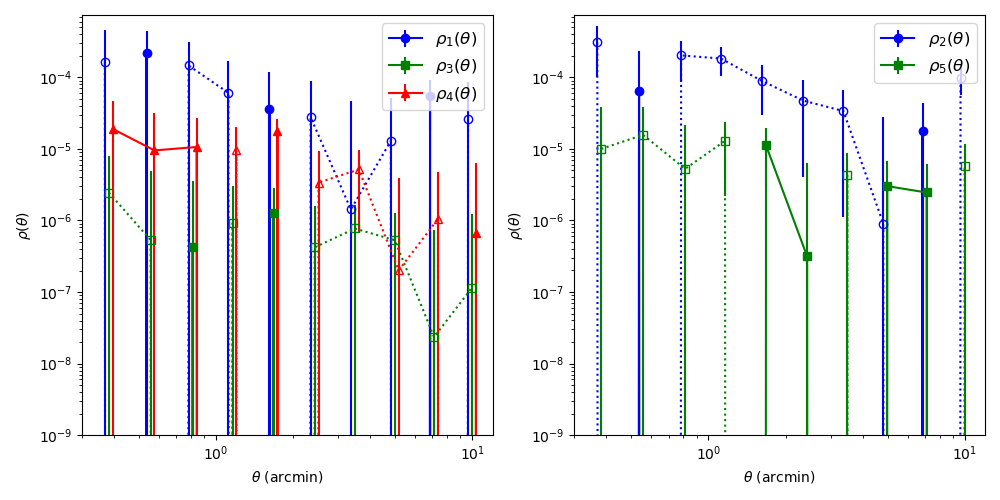
\includegraphics[width=.3\linewidth]{277wControl/piff_rho.png}\hfill
  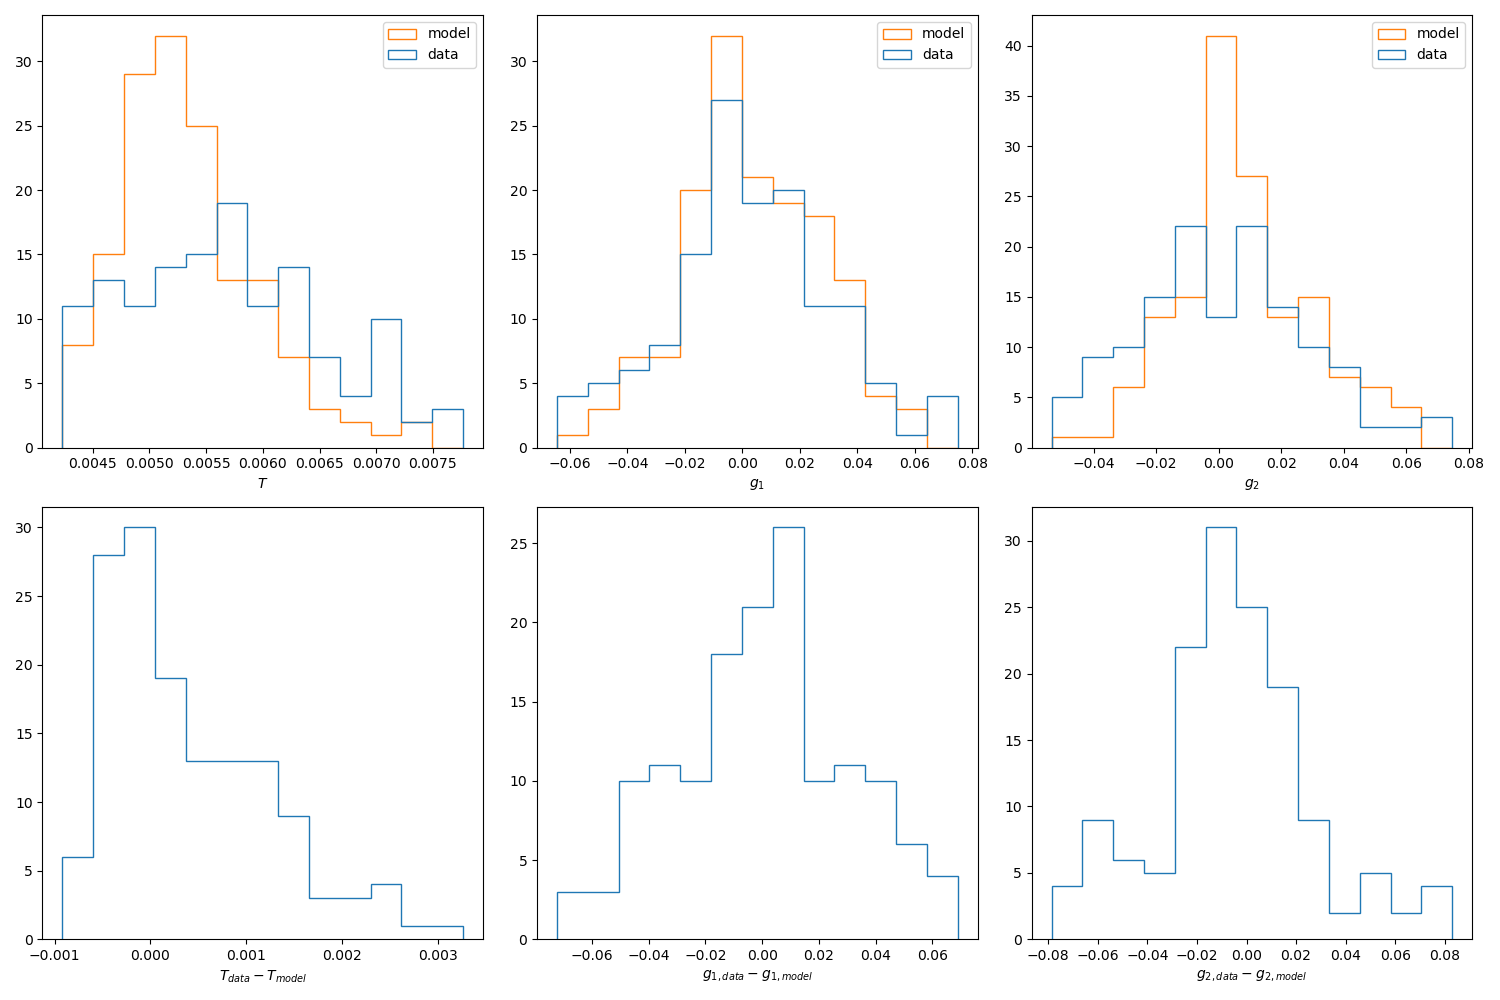
\includegraphics[width=.3\linewidth]{277wControl/piff_shapes.png}\hfill
  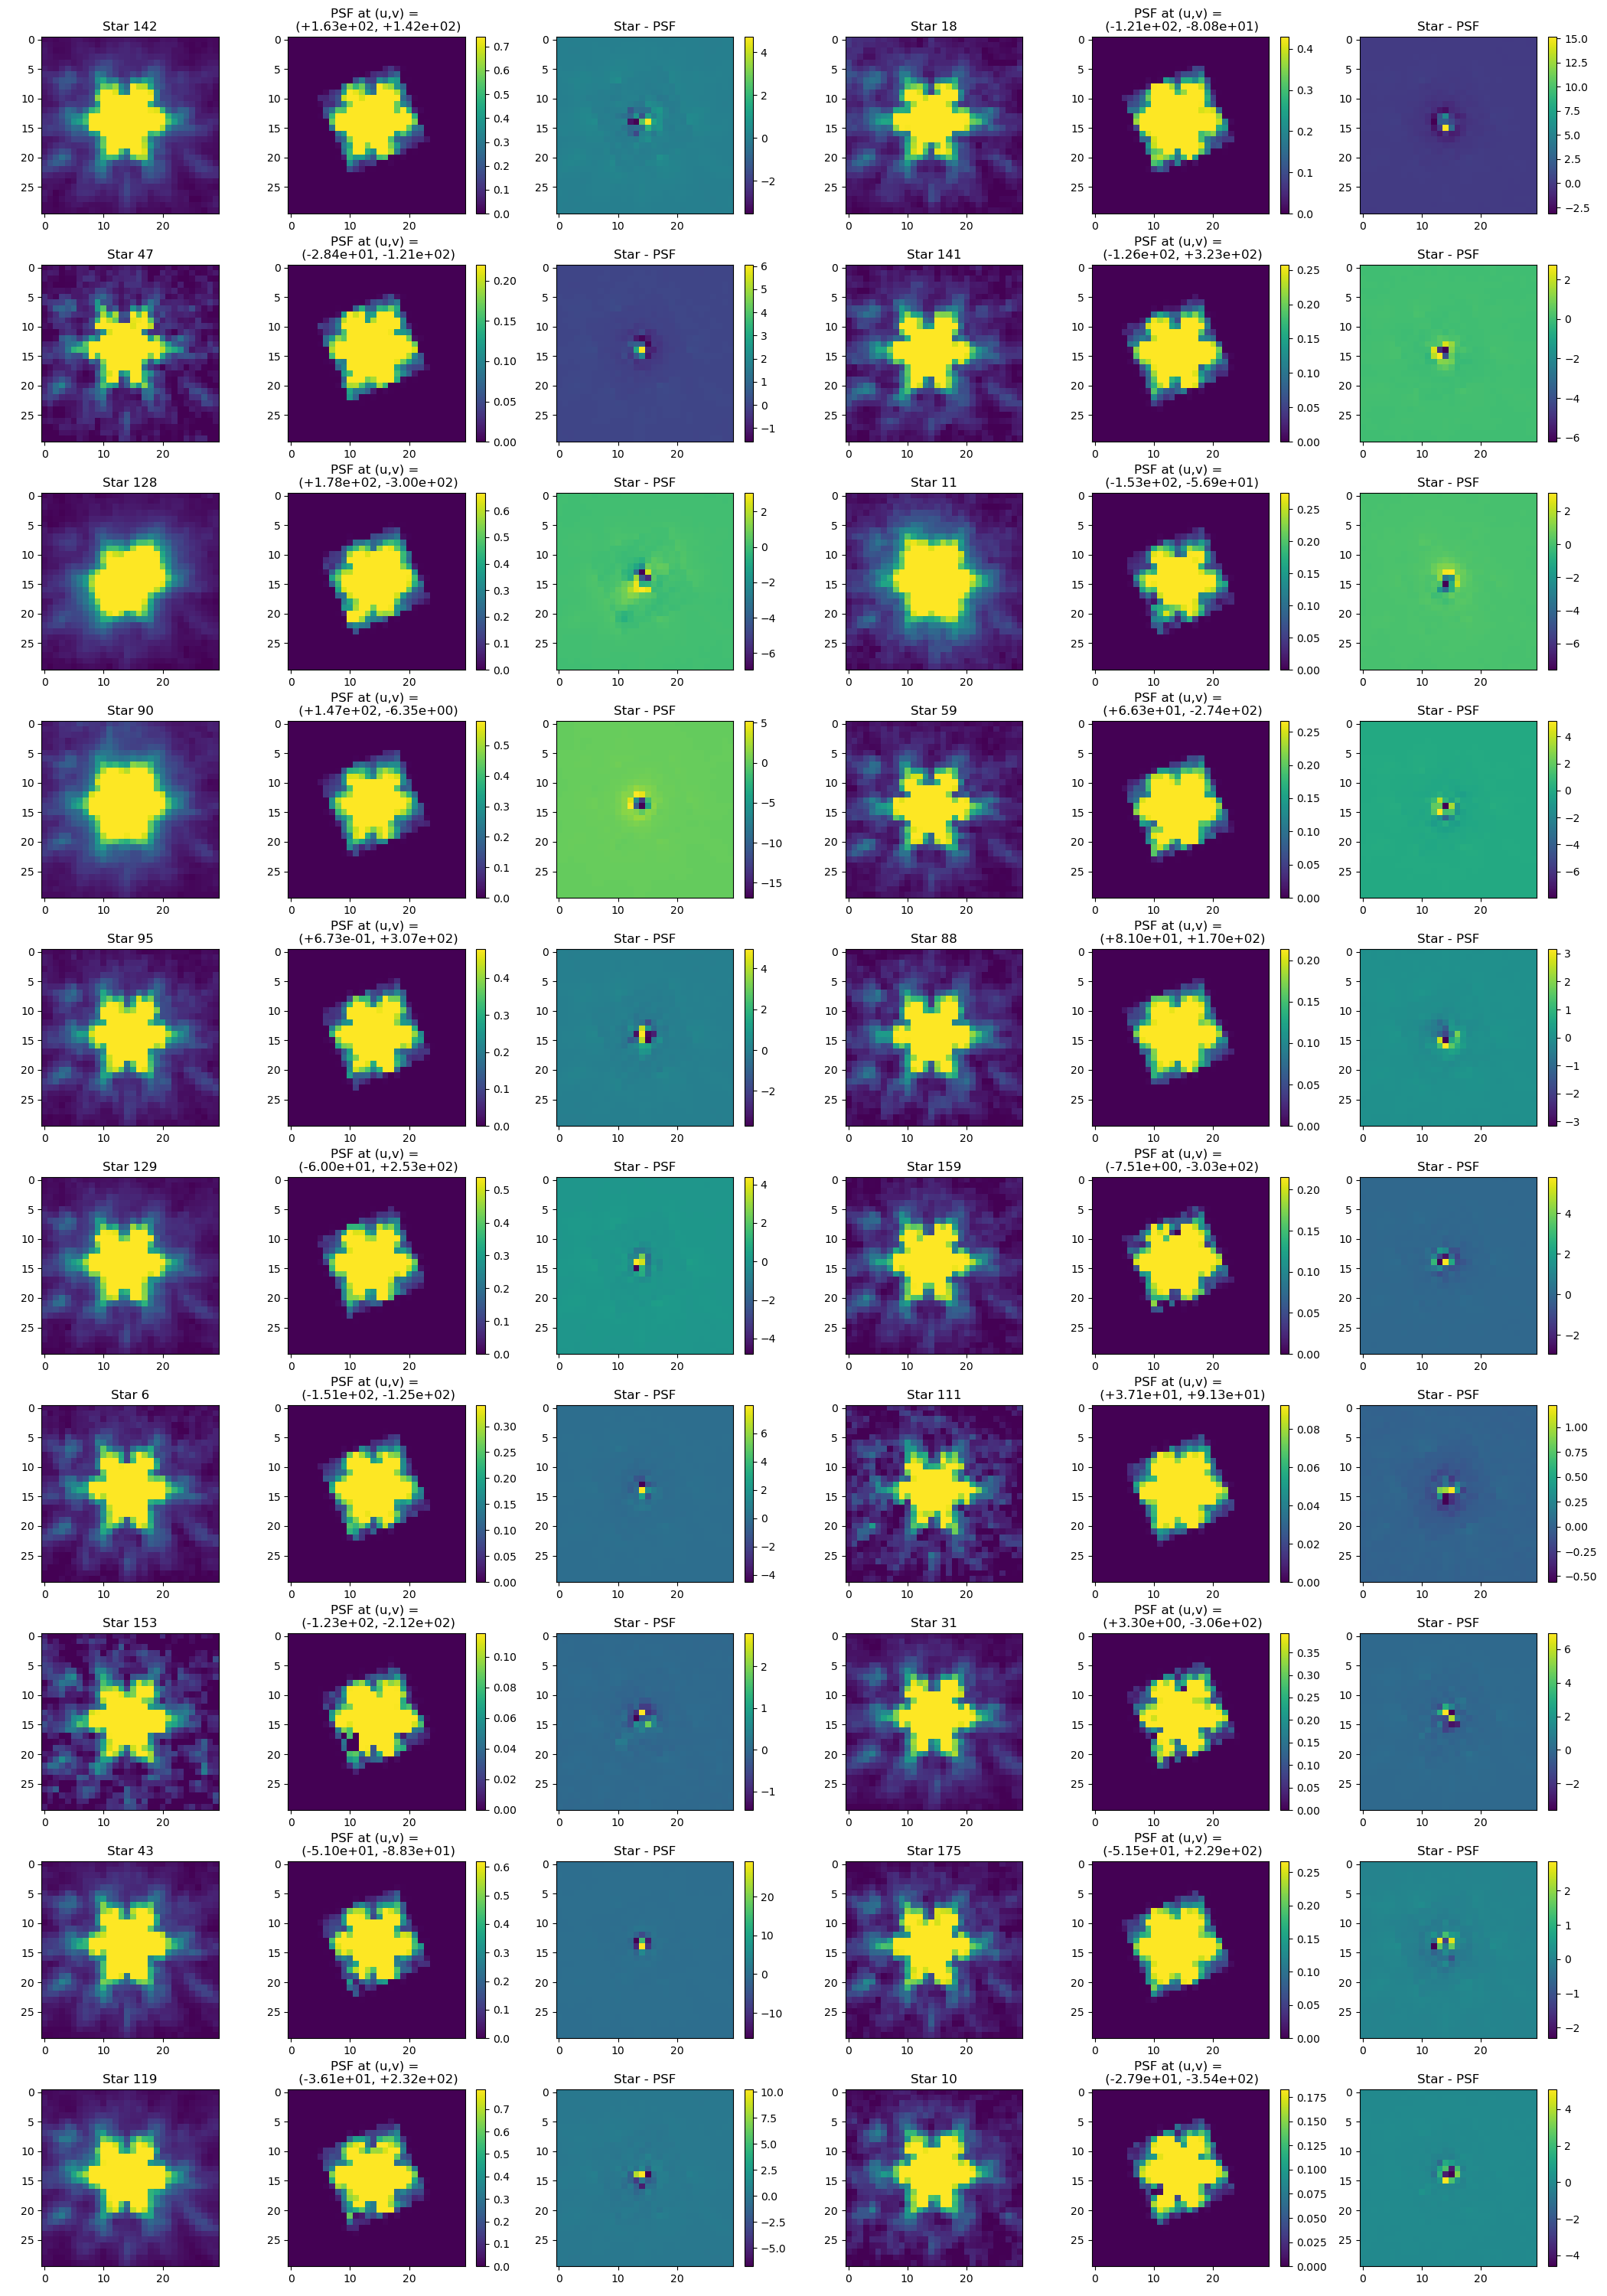
\includegraphics[width=.3\linewidth]{277wControl/piff_stars.png}
  \end{subfigure}\par\medskip
  \begin{subfigure}{\linewidth}
  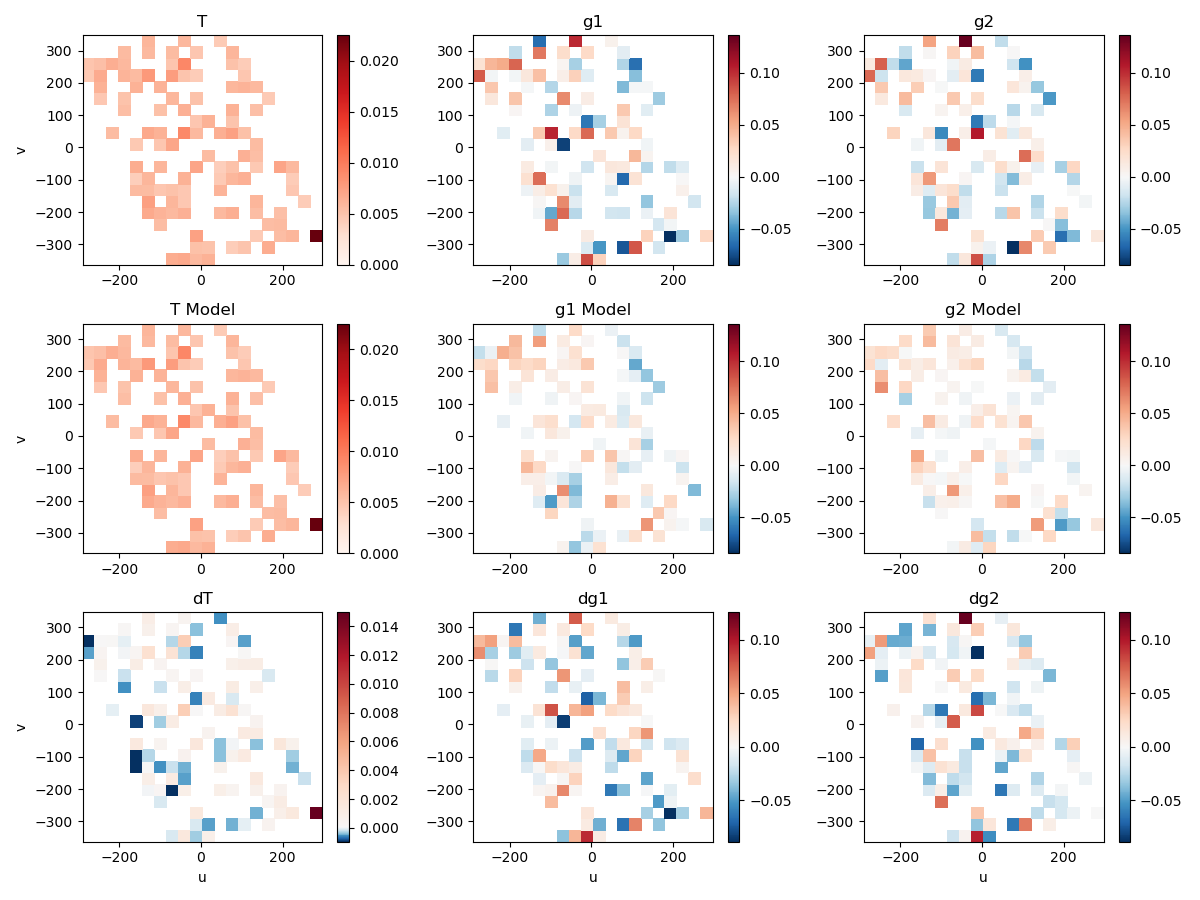
\includegraphics[width=.3\linewidth]{277wControl/piff_twod.png}\hfill
  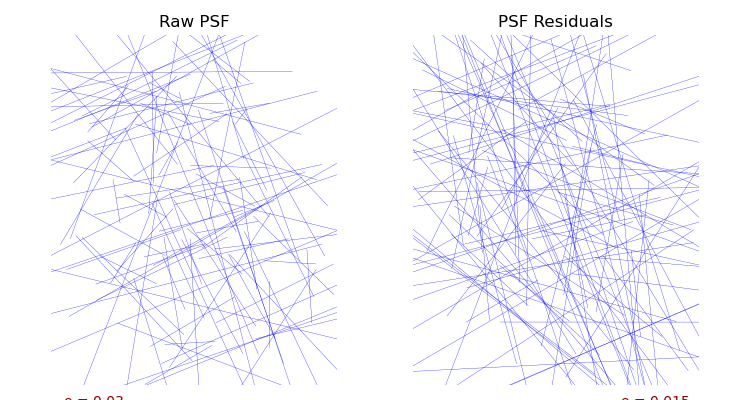
\includegraphics[width=.3\linewidth]{277wControl/piff_whisker.png}\hfill
  \caption{f227w Control}
  \end{subfigure}\par\medskip


\end{figure}

\begin{figure}[!]
  \begin{subfigure}{\linewidth}
  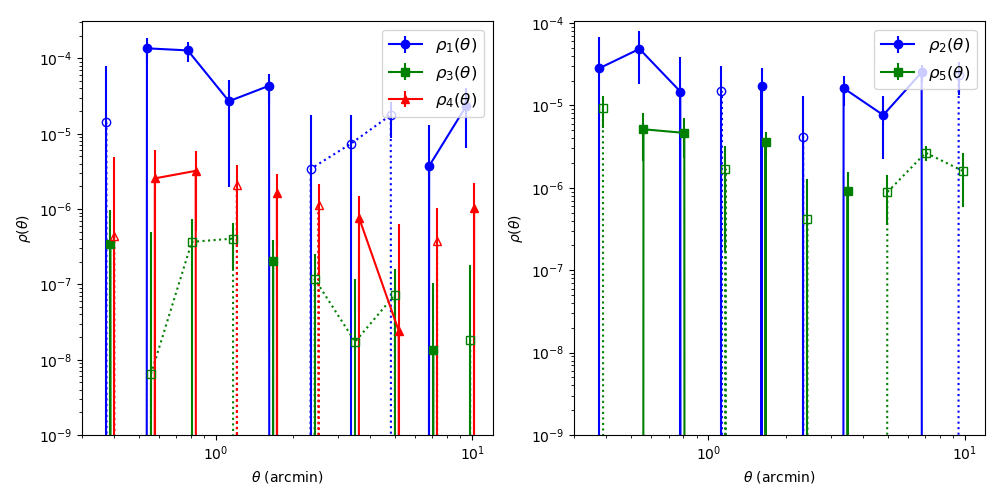
\includegraphics[width=.3\linewidth]{444wControl/piff_rho.png}\hfill
  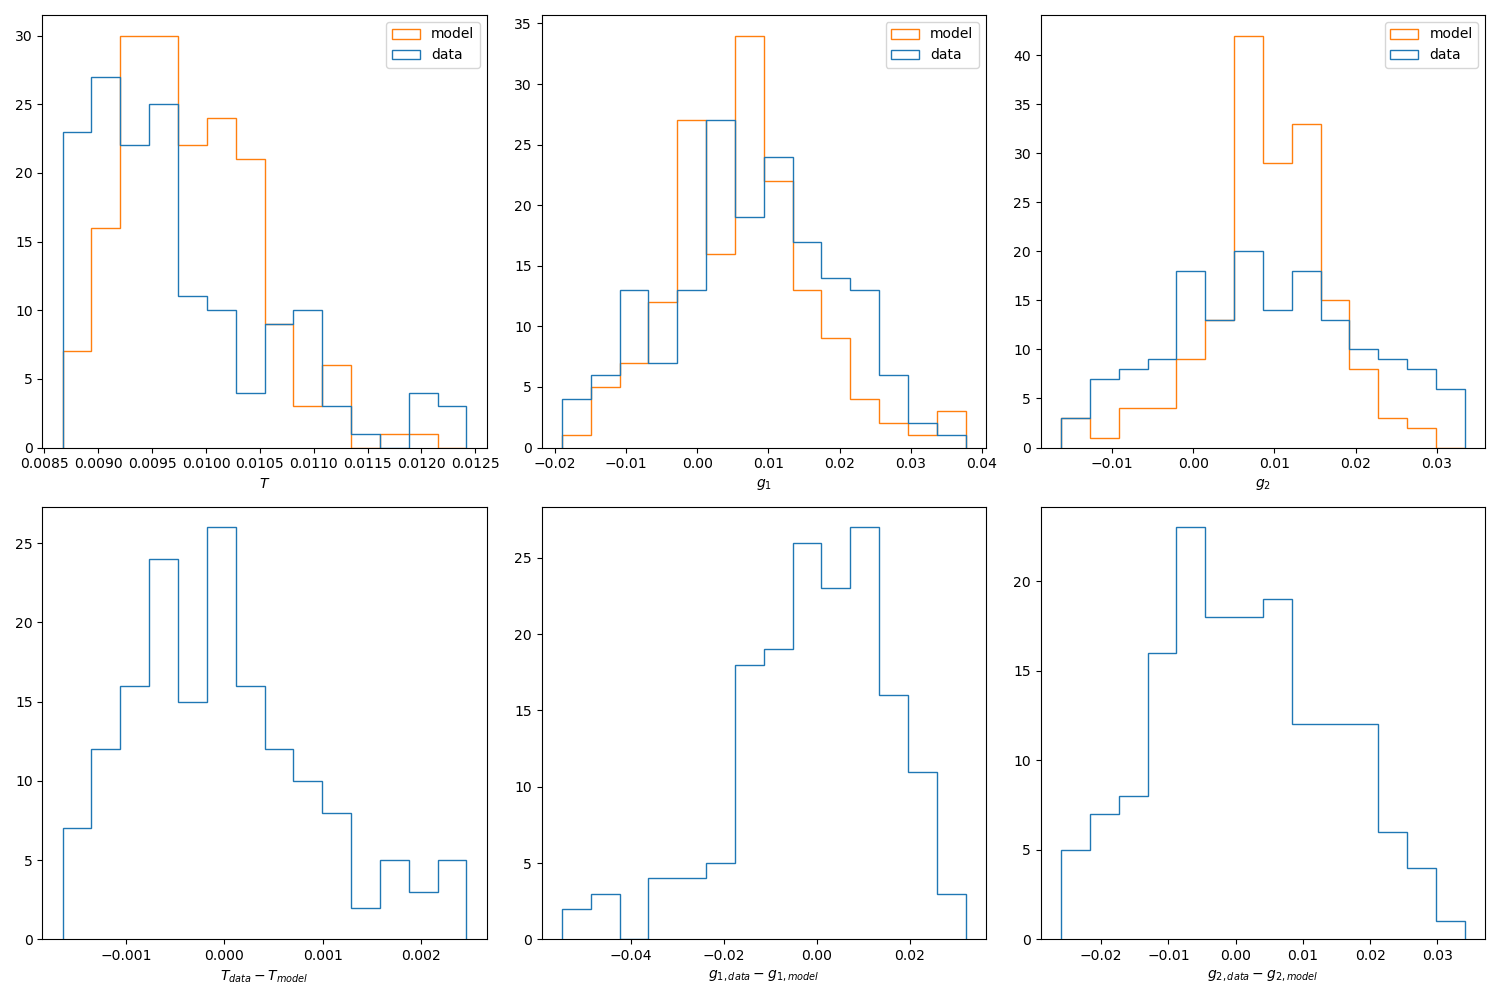
\includegraphics[width=.3\linewidth]{444wControl/piff_shapes.png}\hfill
  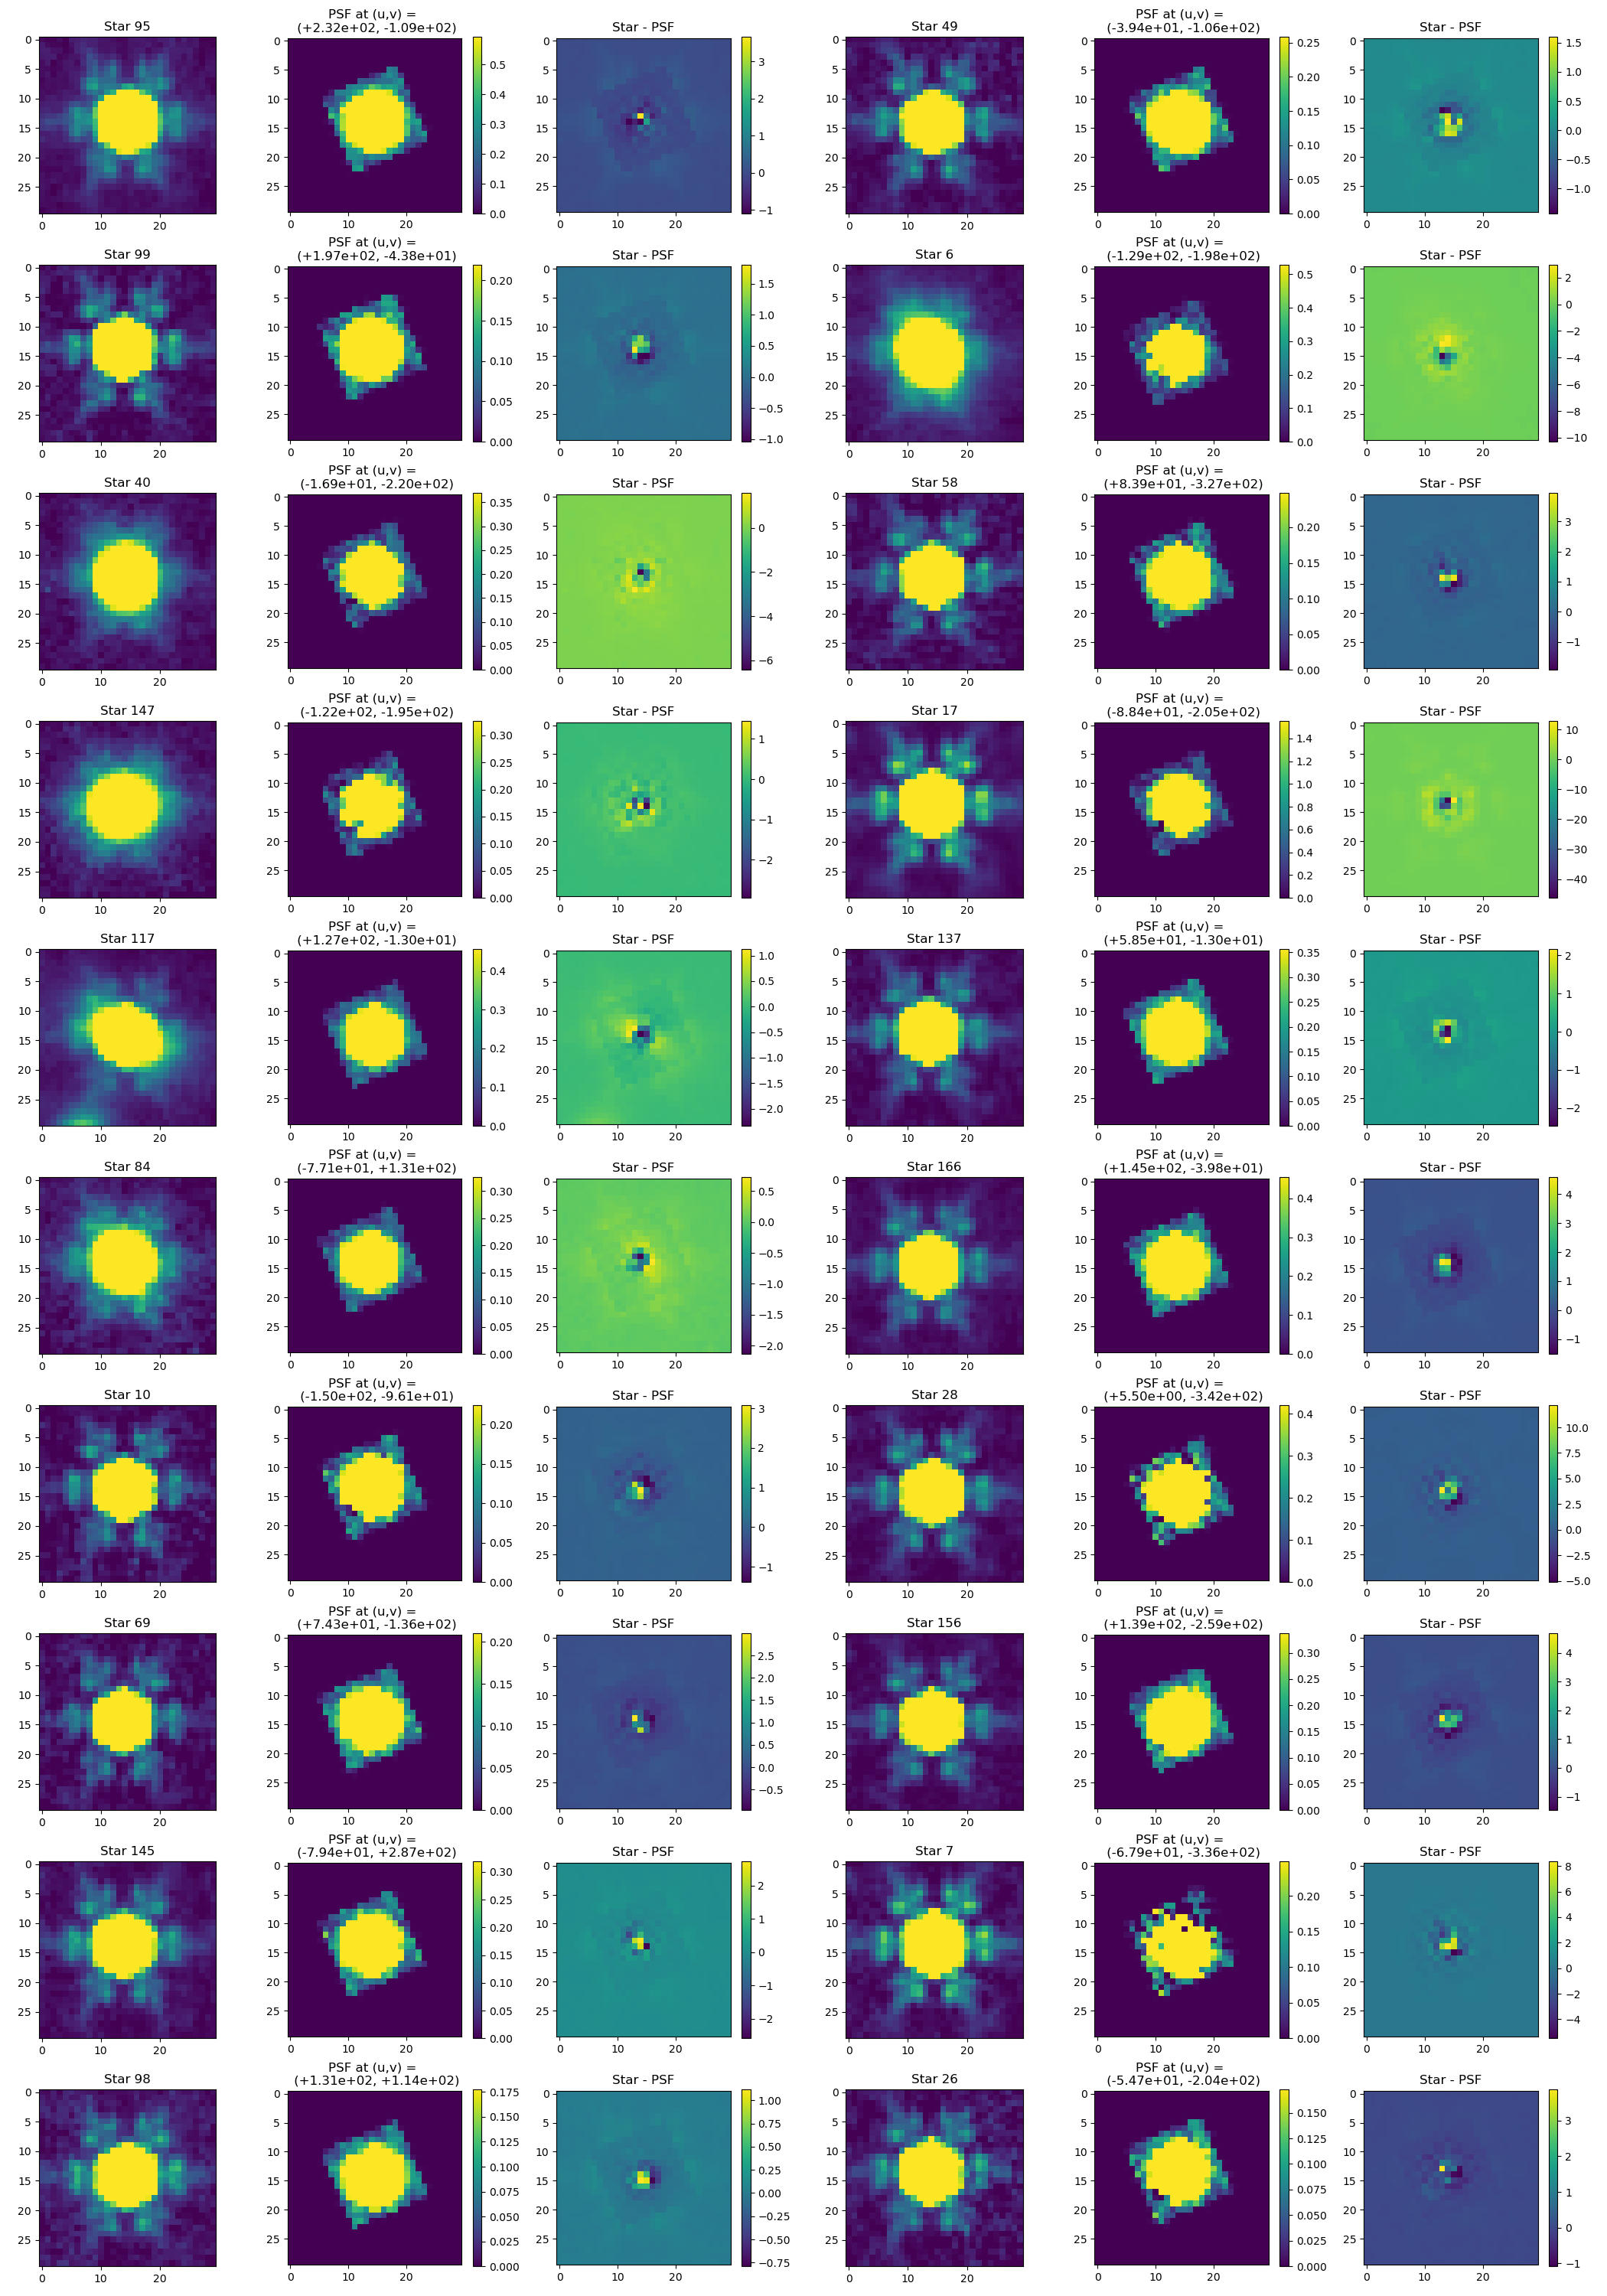
\includegraphics[width=.3\linewidth]{444wControl/piff_stars.png}
  \end{subfigure}\par\medskip
  \begin{subfigure}{\linewidth}
  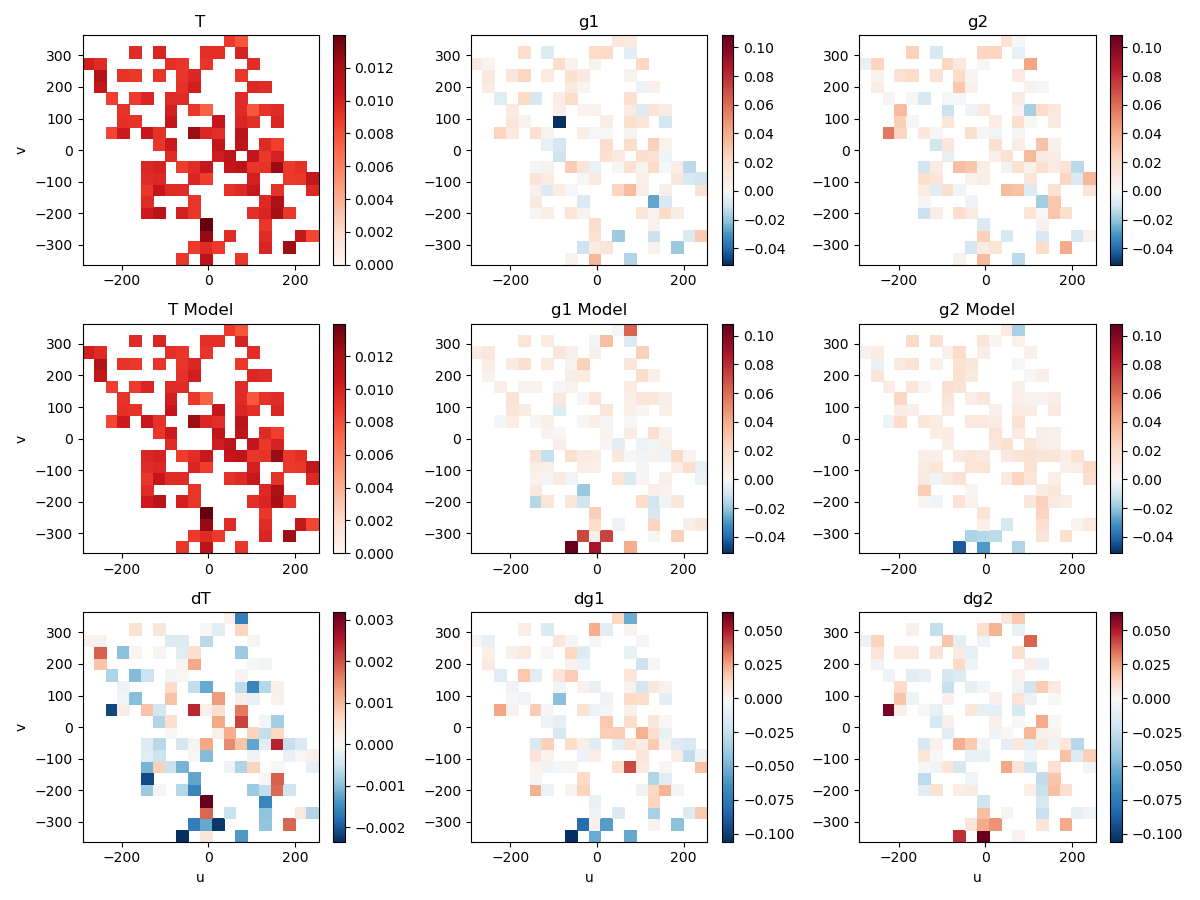
\includegraphics[width=.3\linewidth]{444wControl/piff_twod.png}\hfill
  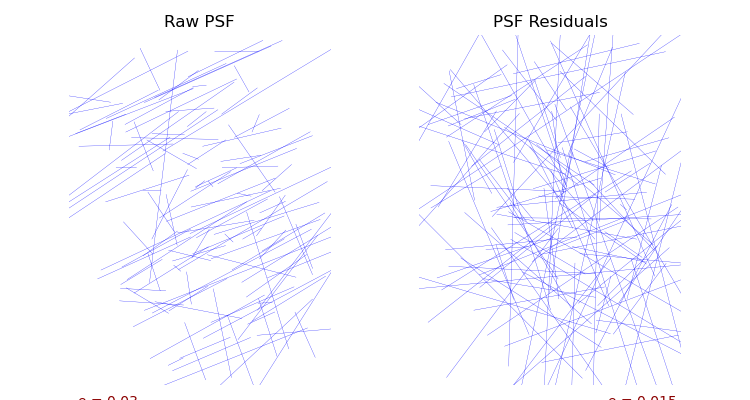
\includegraphics[width=.3\linewidth]{444wControl/piff_whisker.png}\hfill
  \caption{f444w Control}
  \end{subfigure}\par\medskip


\end{figure}
\newpage
\subsection{size change}
\begin{python}
# How large should the postage stamp cutouts of the stars be?
    stamp_size: 30

model:
    # This model uses a grid of pixels to model the surface brightness distribution.
    type: PixelGrid
    scale: 0.025      # NIRCam ative pixel scale
    size: 36          # Model is 24 x 24 in these pixels
\end{python}\\
Failed with F115?\\
\begin{figure}[!h]
  \begin{subfigure}{\linewidth}
  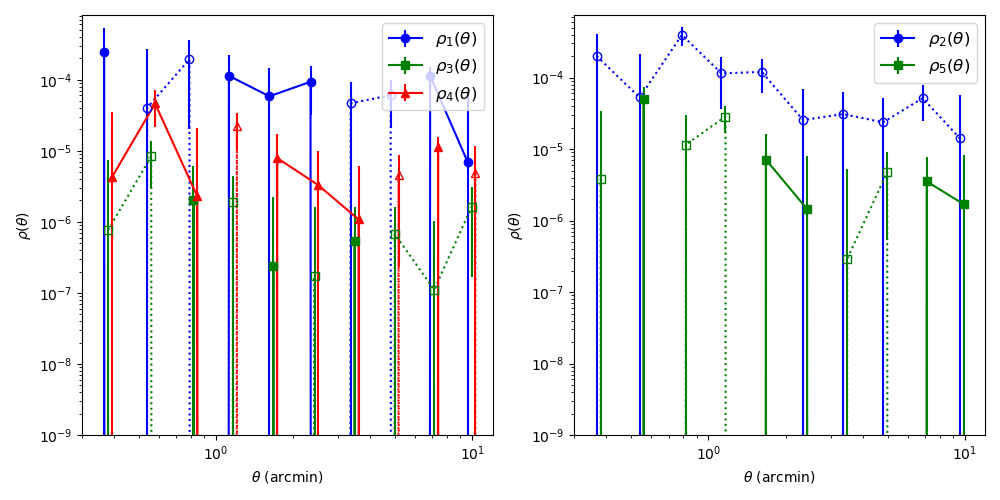
\includegraphics[width=.3\linewidth]{277wSize36/piff_rho.png}\hfill
  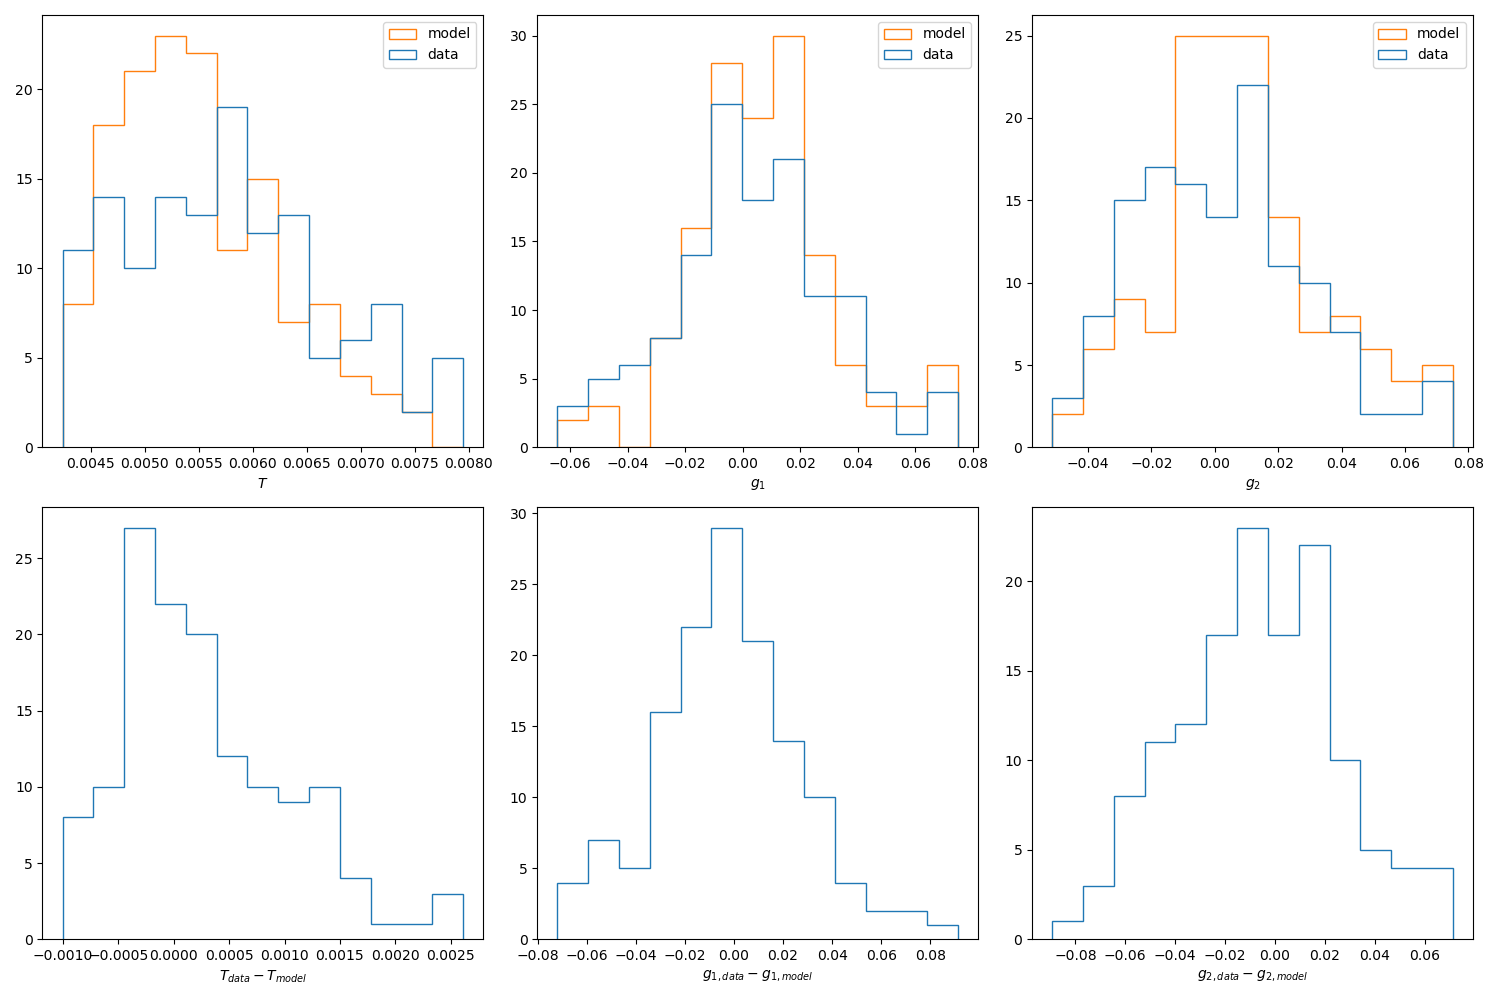
\includegraphics[width=.3\linewidth]{277wSize36/piff_shapes.png}\hfill
  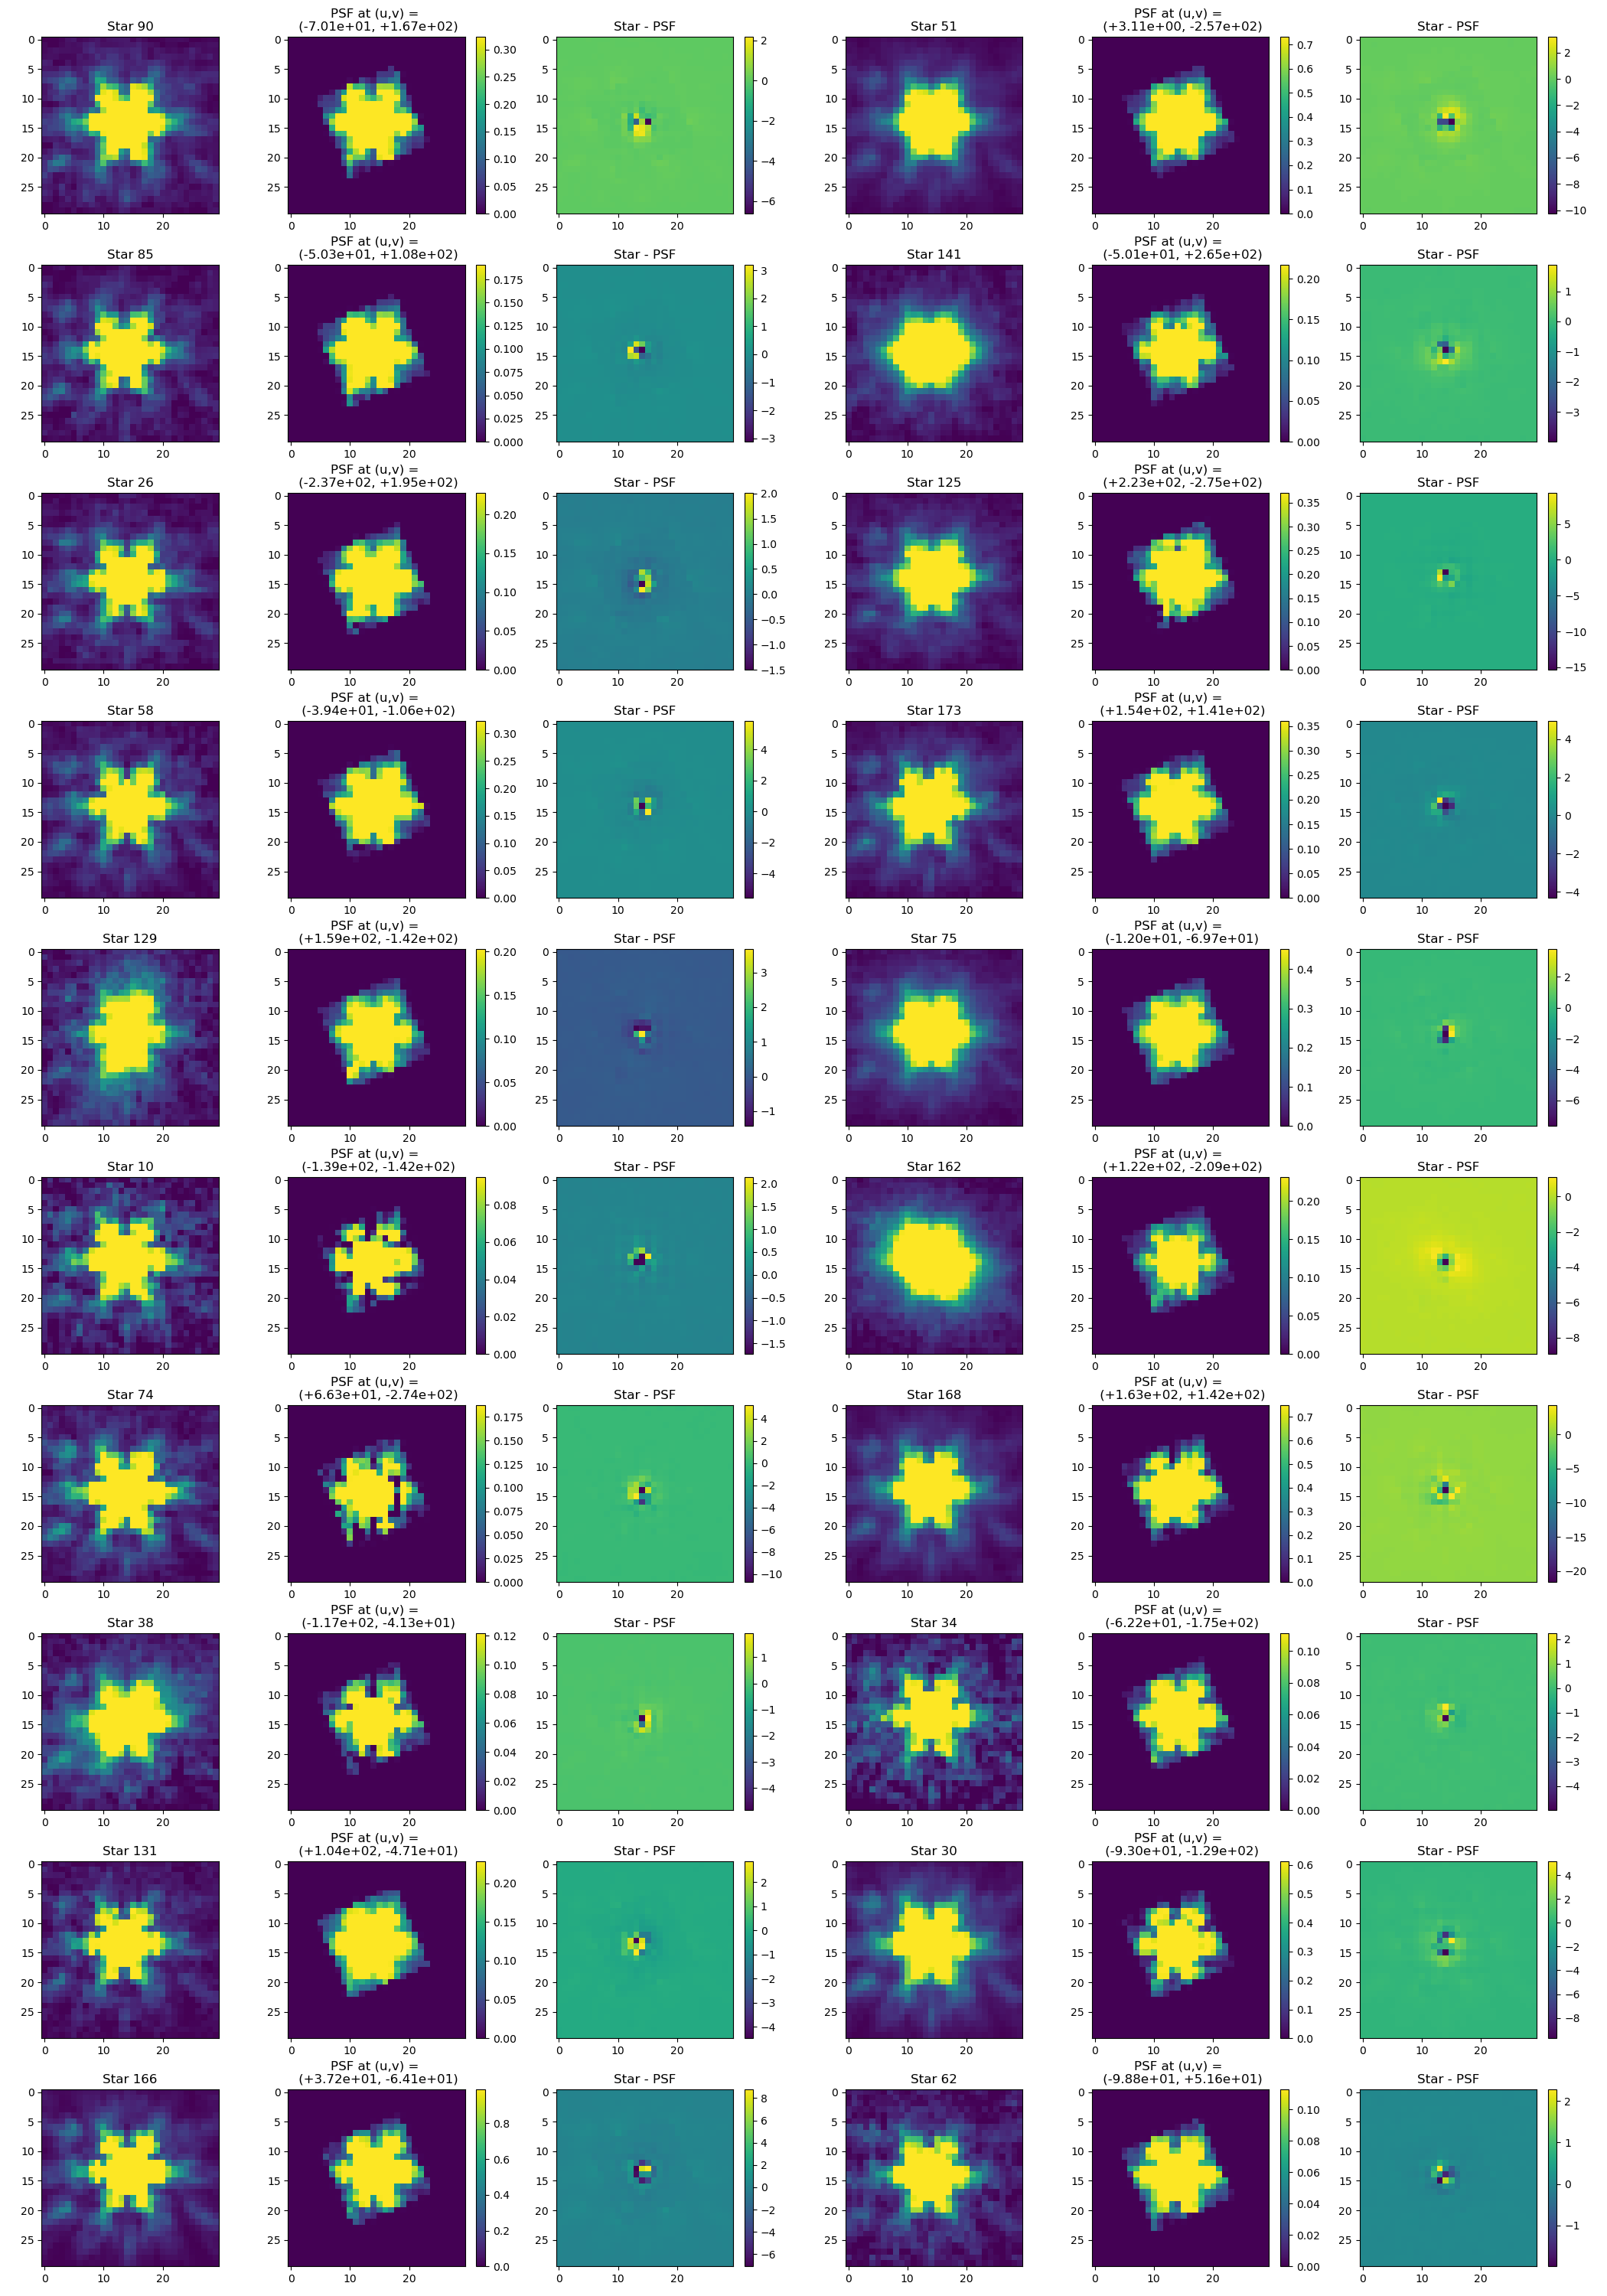
\includegraphics[width=.3\linewidth]{277wSize36/piff_stars.png}
  \end{subfigure}\par\medskip
  \begin{subfigure}{\linewidth}
  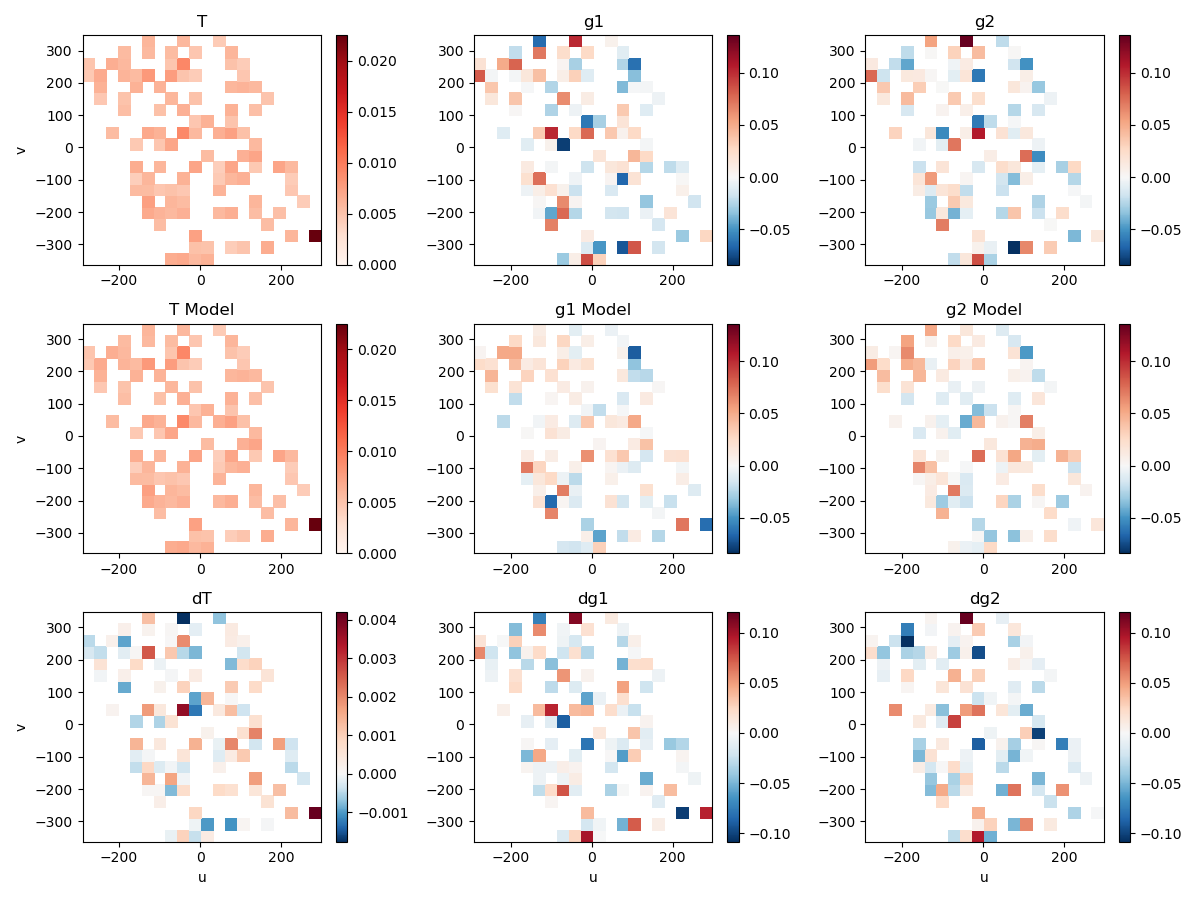
\includegraphics[width=.3\linewidth]{277wSize36/piff_twod.png}\hfill
  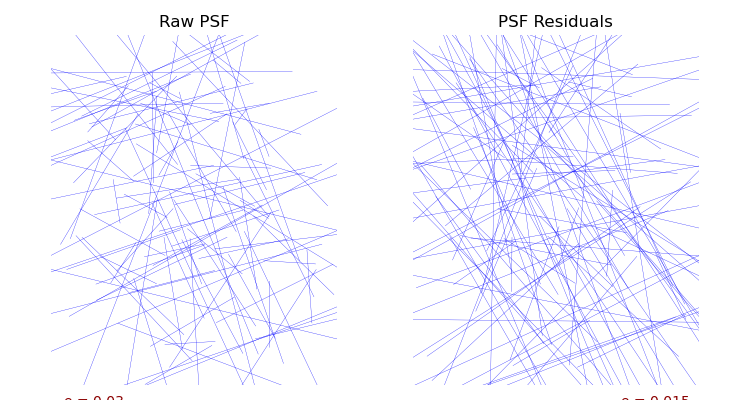
\includegraphics[width=.3\linewidth]{277wSize36/piff_whisker.png}\hfill
  \caption{f277w Size 36}
  \end{subfigure}\par\medskip


\end{figure}\\ 
\newpage
\begin{figure}[!h]
  \begin{subfigure}{\linewidth}
  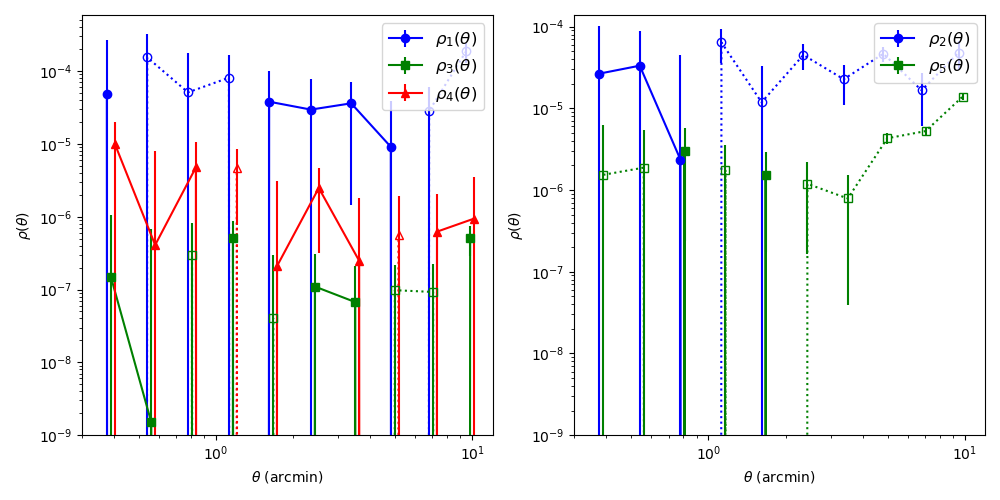
\includegraphics[width=.3\linewidth]{444wSize36/piff_rho.png}\hfill
  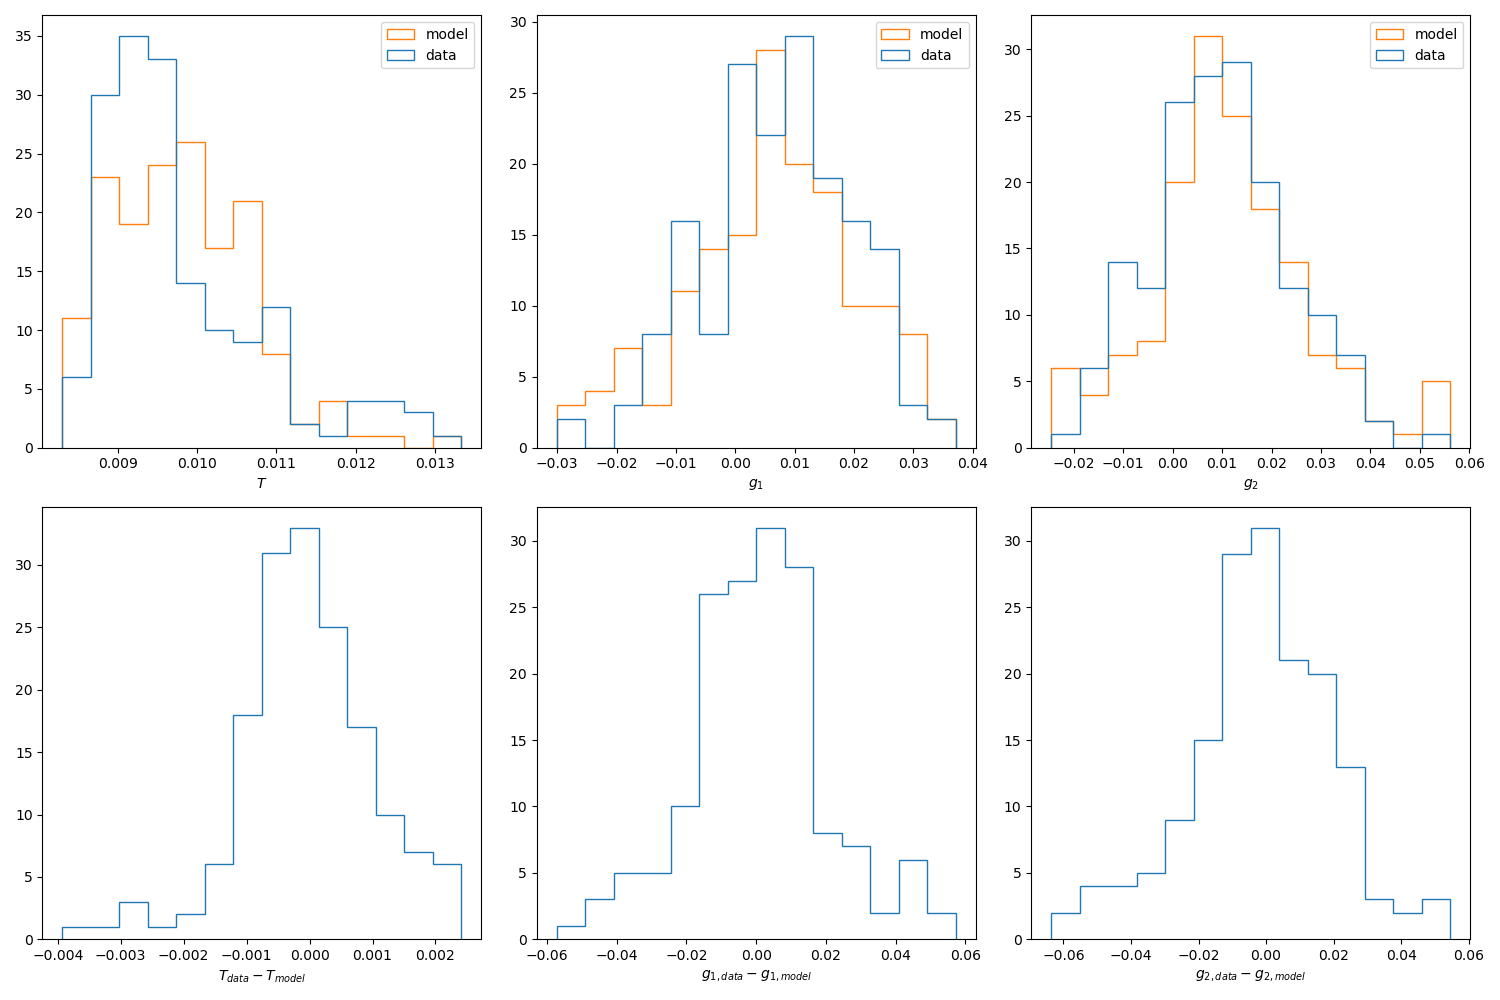
\includegraphics[width=.3\linewidth]{444wSize36/piff_shapes.png}\hfill
  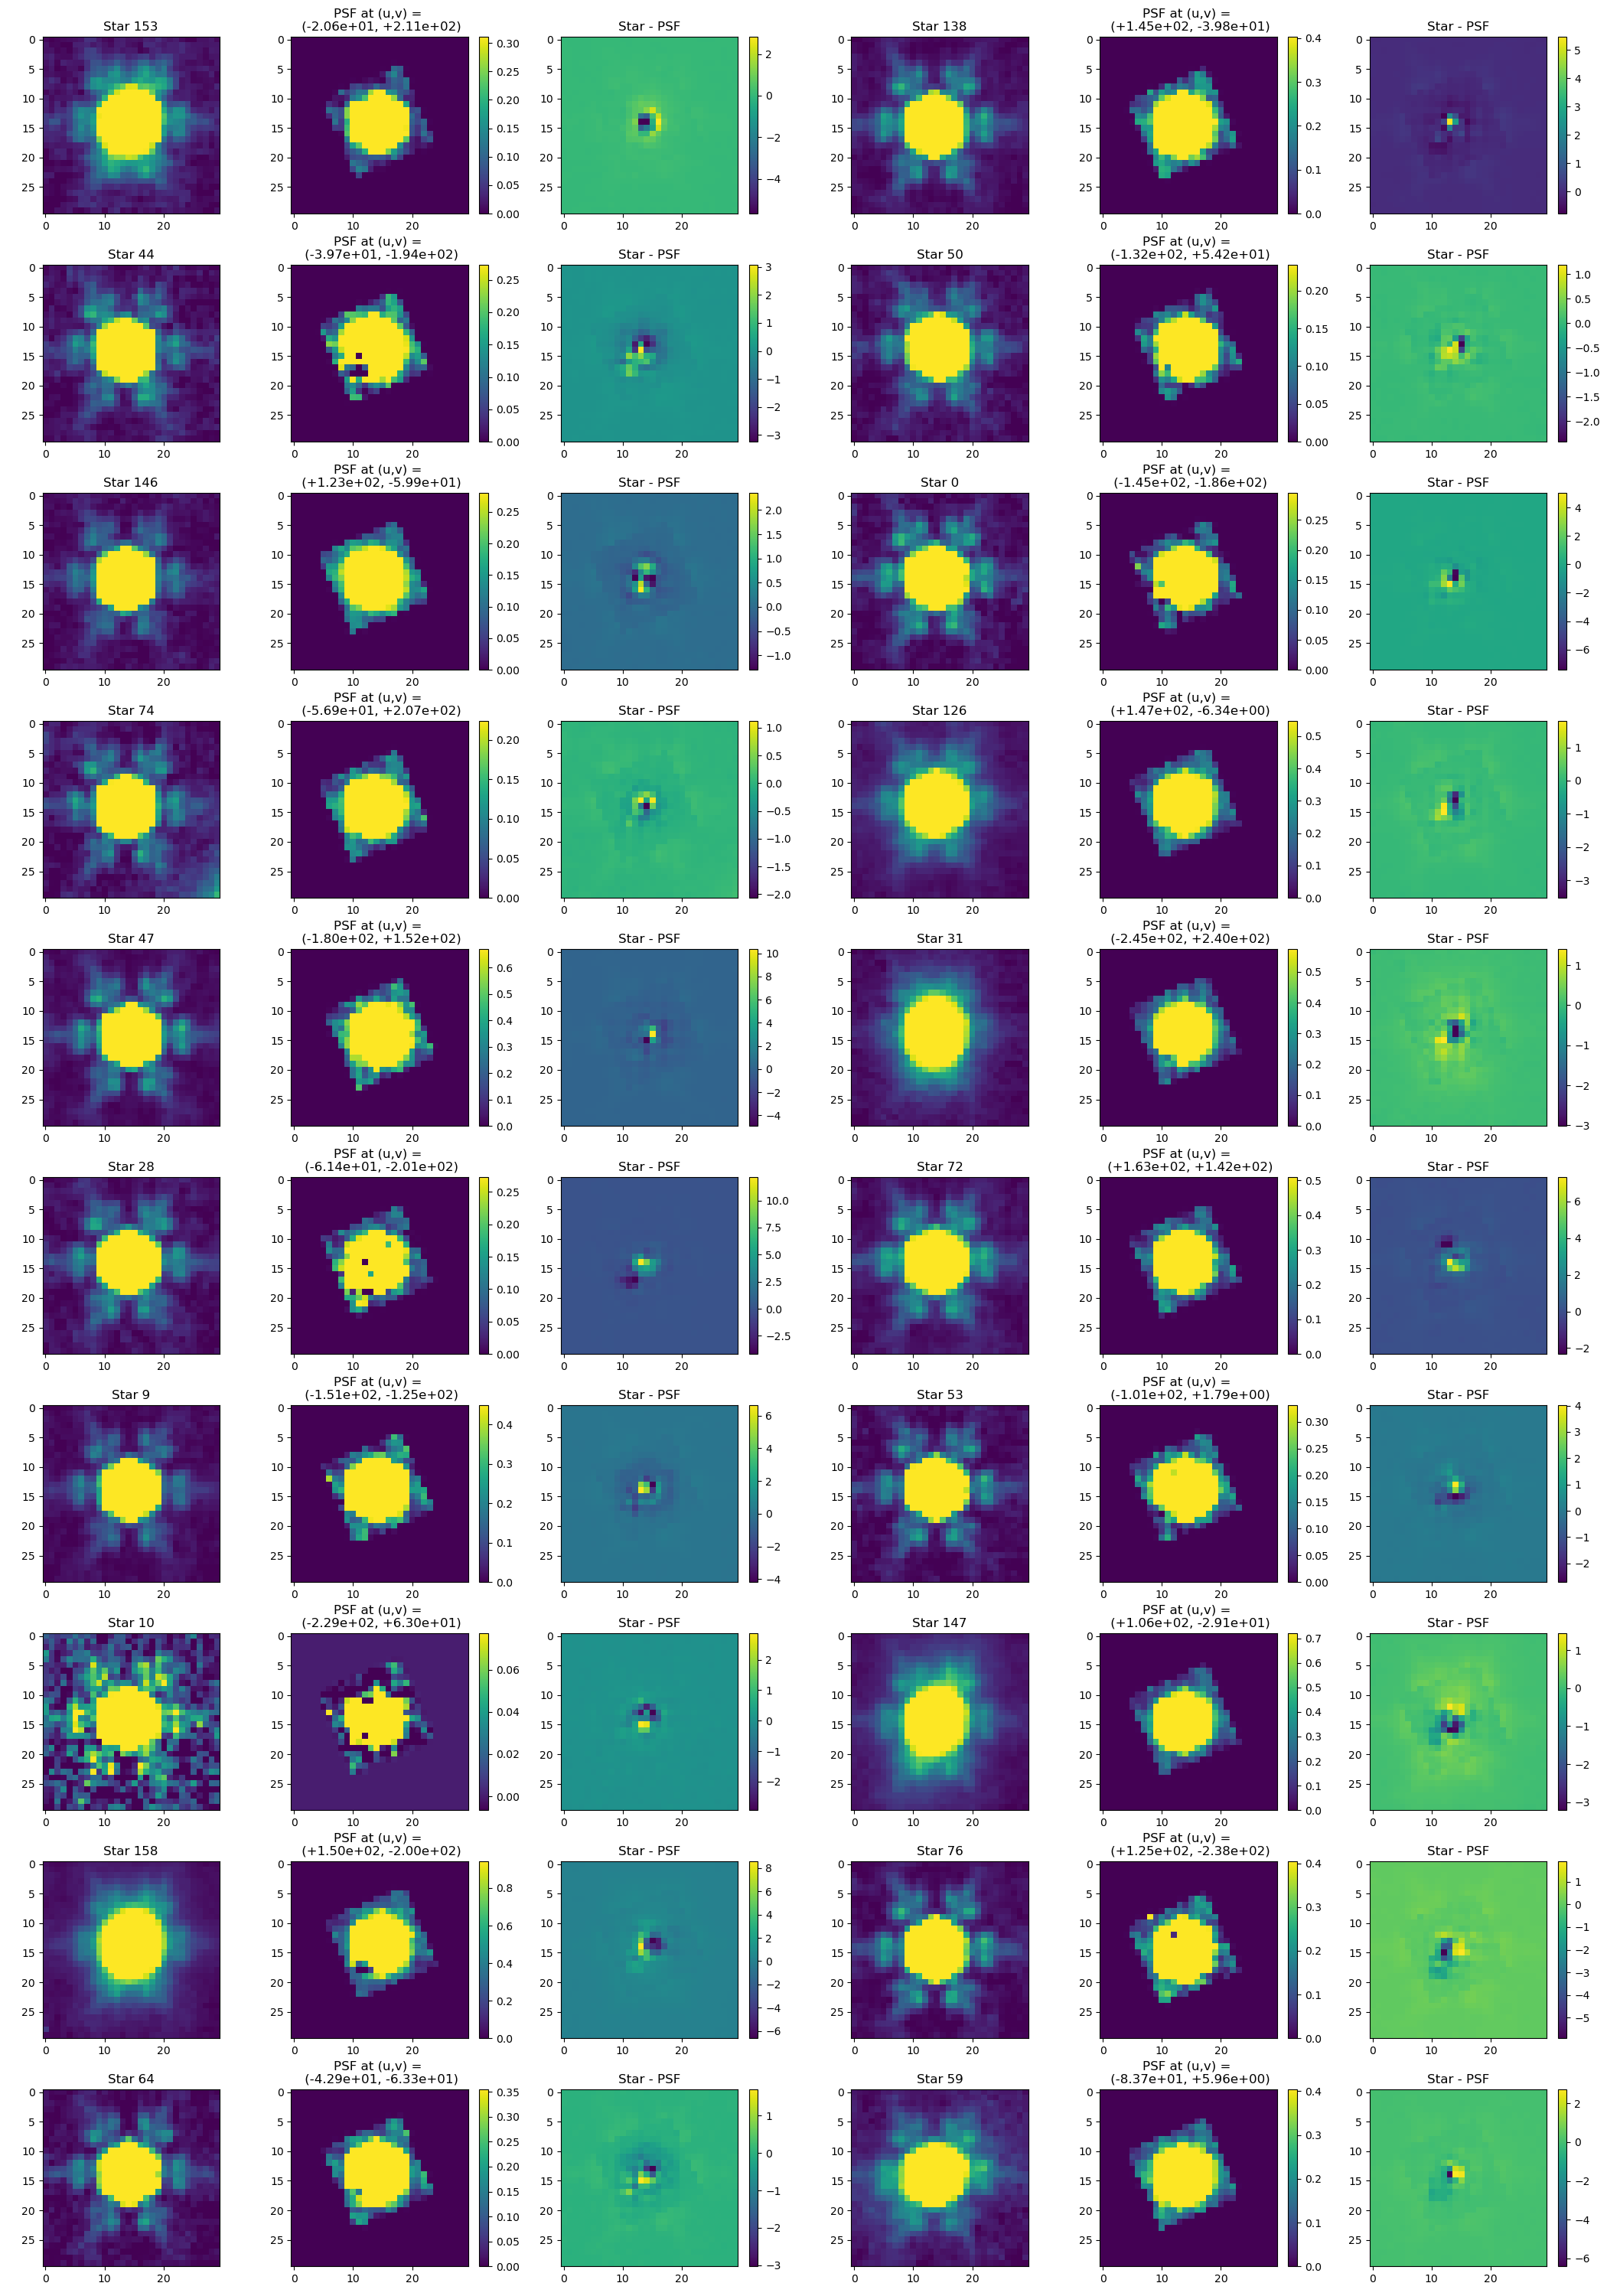
\includegraphics[width=.3\linewidth]{444wSize36/piff_stars.png}
  \end{subfigure}\par\medskip
  \begin{subfigure}{\linewidth}
  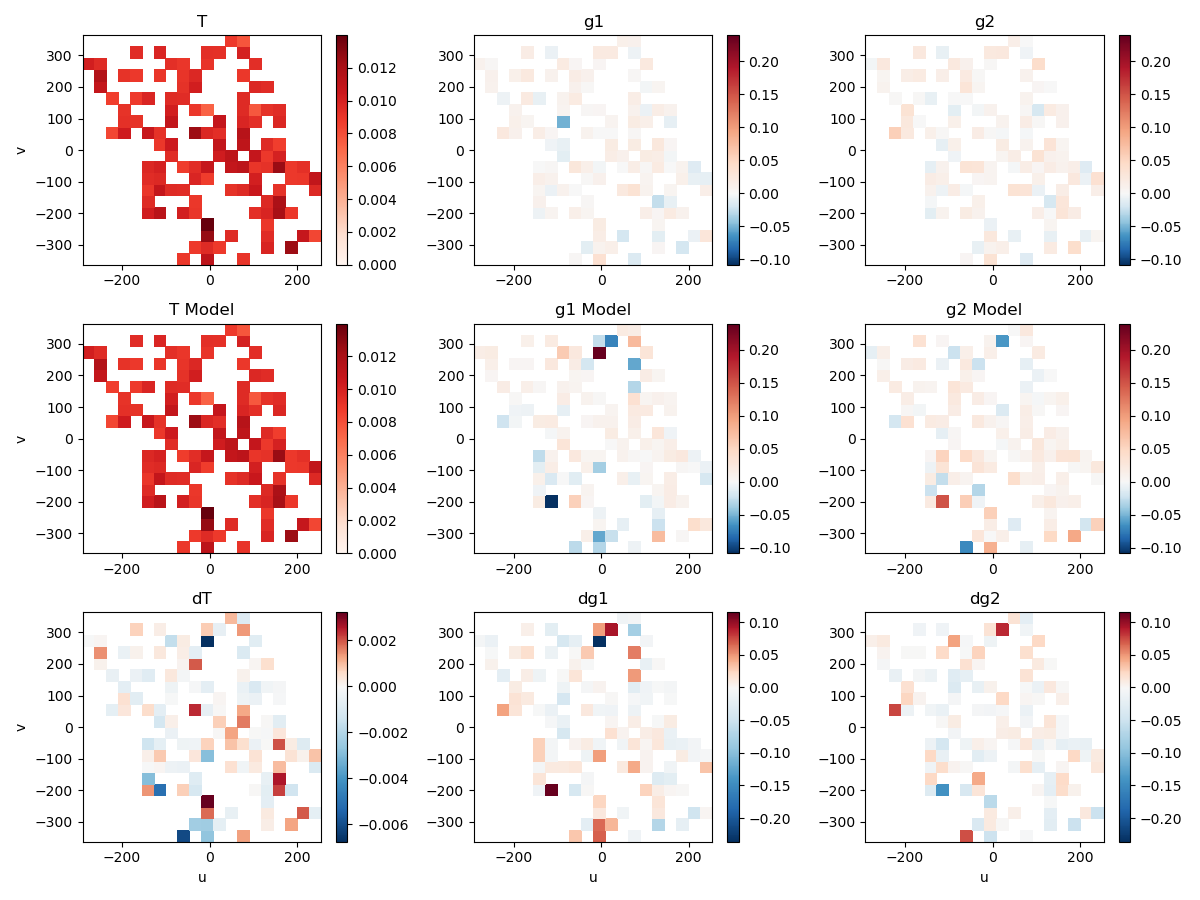
\includegraphics[width=.3\linewidth]{444wSize36/piff_twod.png}\hfill
  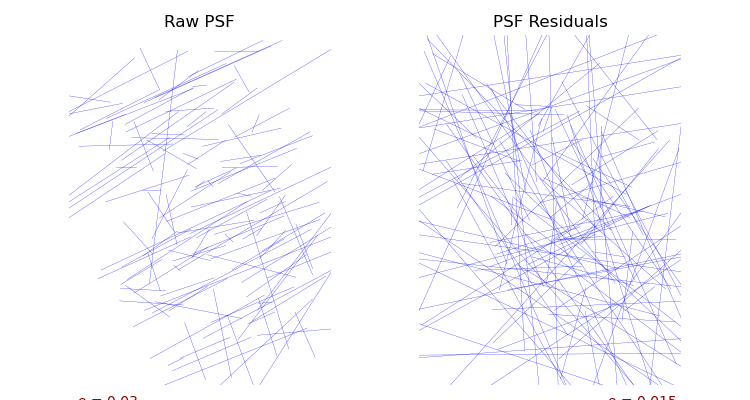
\includegraphics[width=.3\linewidth]{444wSize36/piff_whisker.png}\hfill
  \caption{f444w Size 36}
  \end{subfigure}\par\medskip


\end{figure}\\ 
\newpage
\subsection{Even-Oddness Model Size}
\begin{python}
# How large should the postage stamp cutouts of the stars be?
    stamp_size: 30

model:
    # This model uses a grid of pixels to model the surface brightness distribution.
    type: PixelGrid
    scale: 0.034      # NIRCam ative pixel scale
    size: 27          # Model is 24 x 24 in these pixels
\end{python}\\

\begin{figure}[!h]
  \begin{subfigure}{\linewidth}
  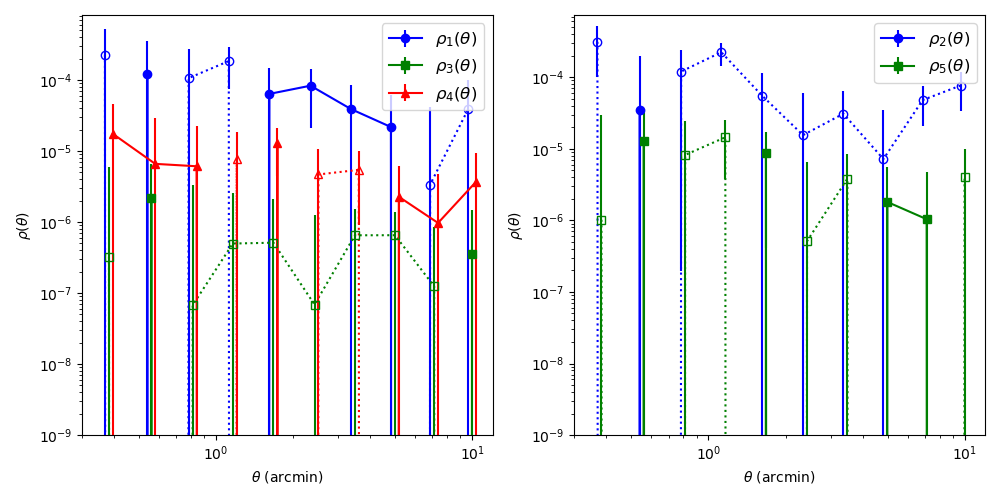
\includegraphics[width=.3\linewidth]{277wOdd/piff_rho.png}\hfill
  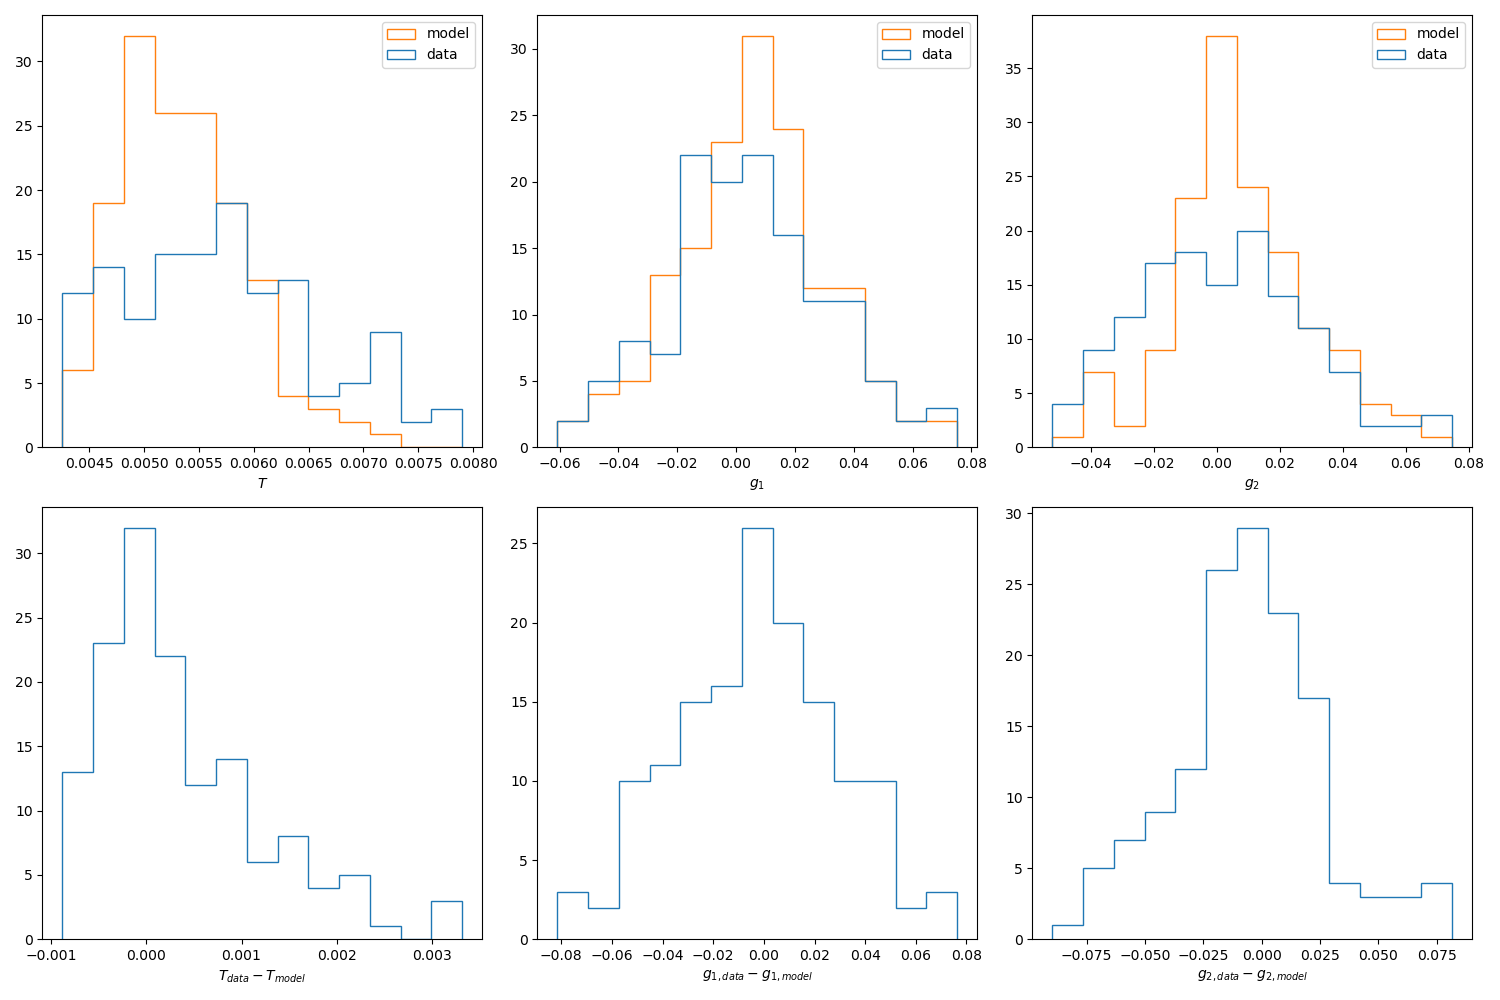
\includegraphics[width=.3\linewidth]{277wOdd/piff_shapes.png}\hfill
  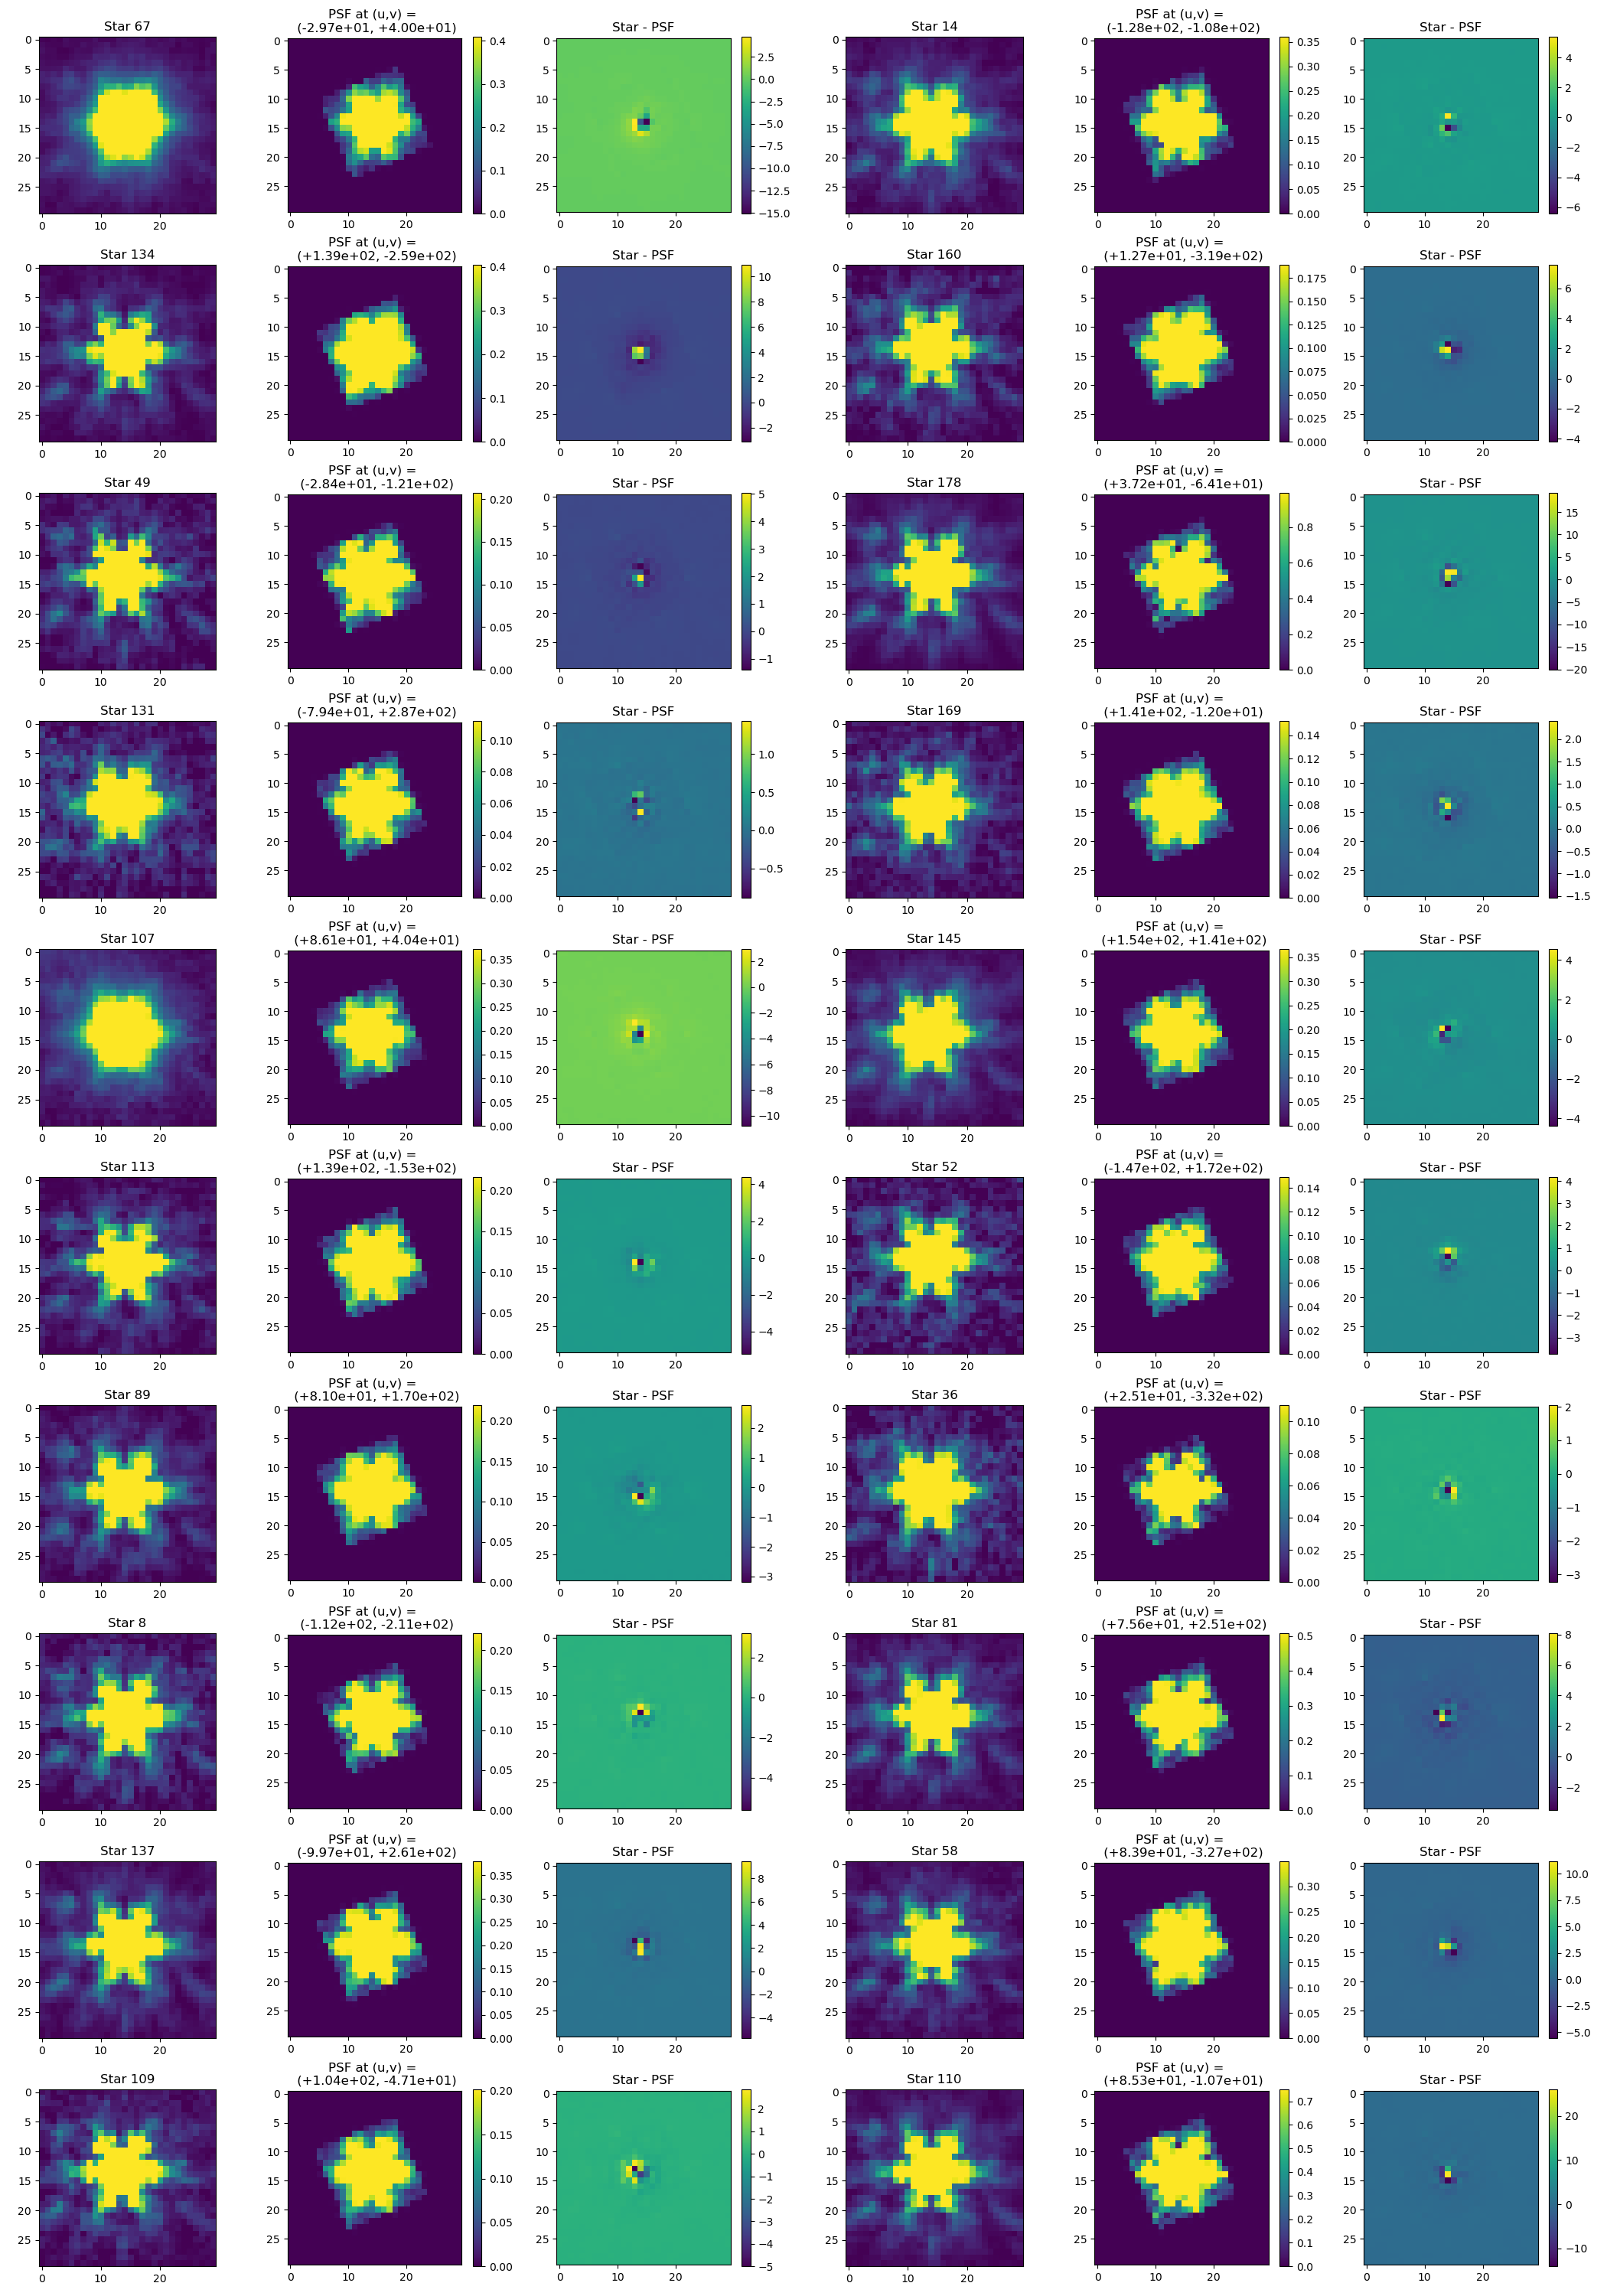
\includegraphics[width=.3\linewidth]{277wOdd/piff_stars.png}
  \end{subfigure}\par\medskip
  \begin{subfigure}{\linewidth}
  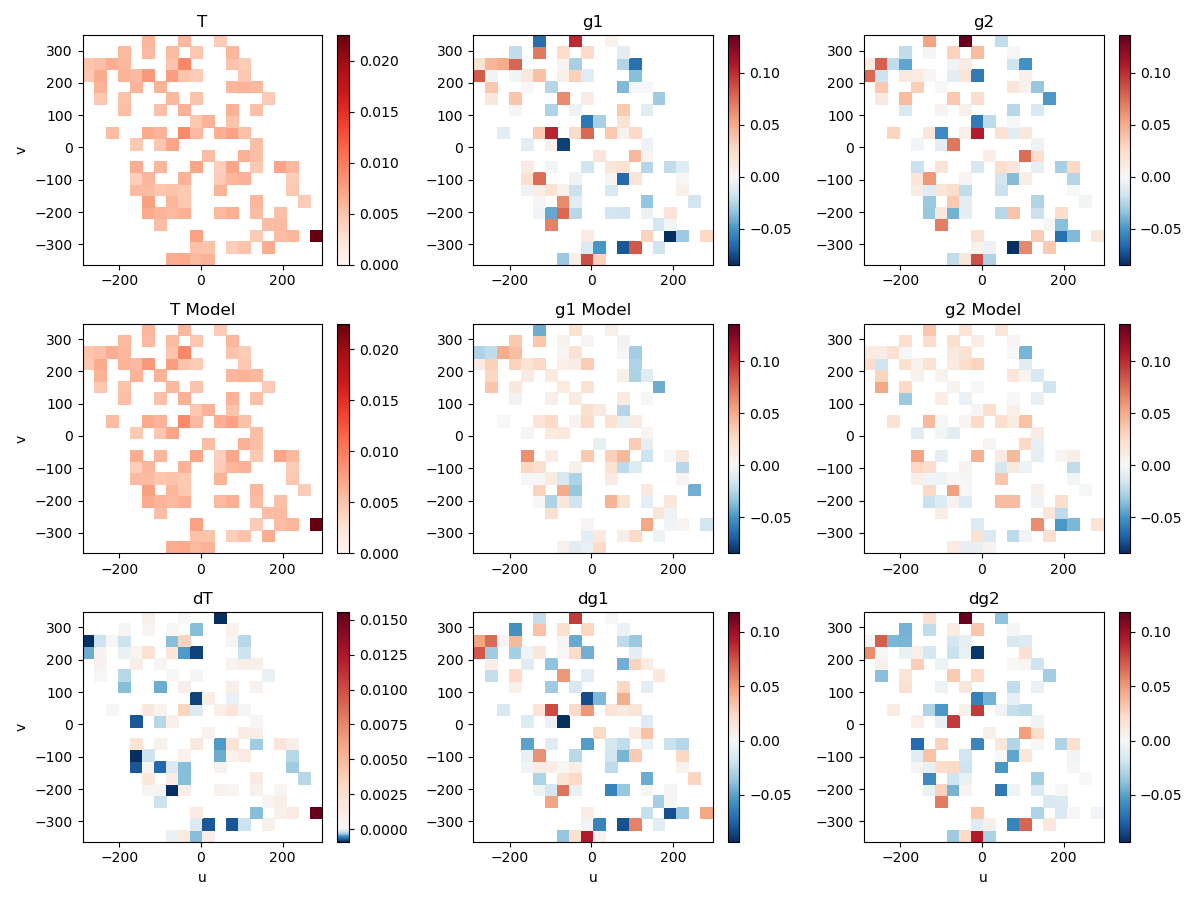
\includegraphics[width=.3\linewidth]{277wOdd/piff_twod.png}\hfill
  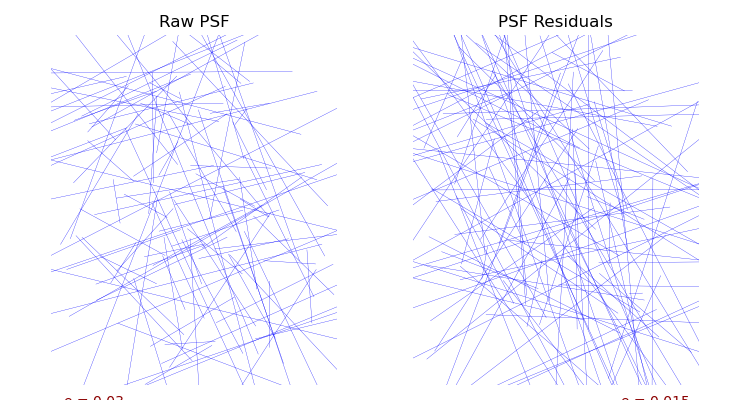
\includegraphics[width=.3\linewidth]{277wOdd/piff_whisker.png}\hfill
  \caption{f277w Odd Model Size}
  \end{subfigure}\par\medskip
\end{figure}\\ 

\begin{figure}[!h]
  \begin{subfigure}{\linewidth}
  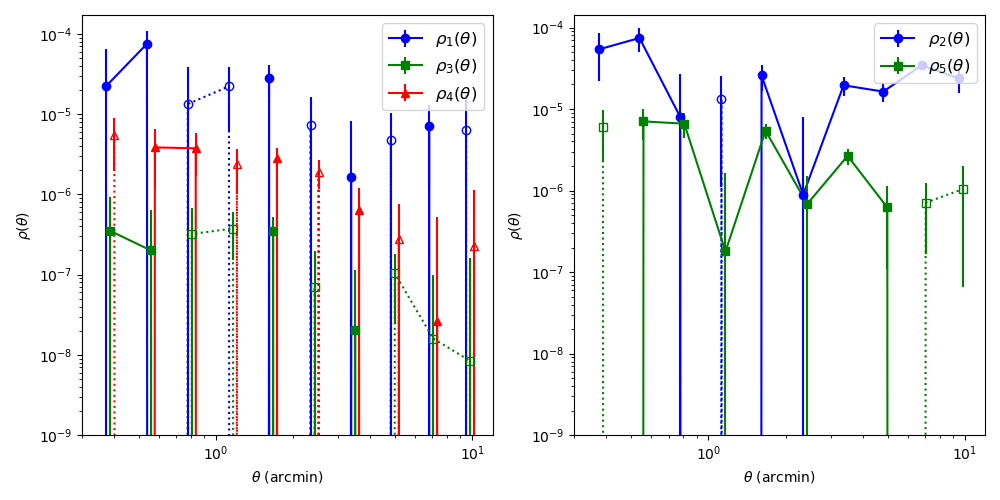
\includegraphics[width=.3\linewidth]{444wOdd/piff_rho.png}\hfill
  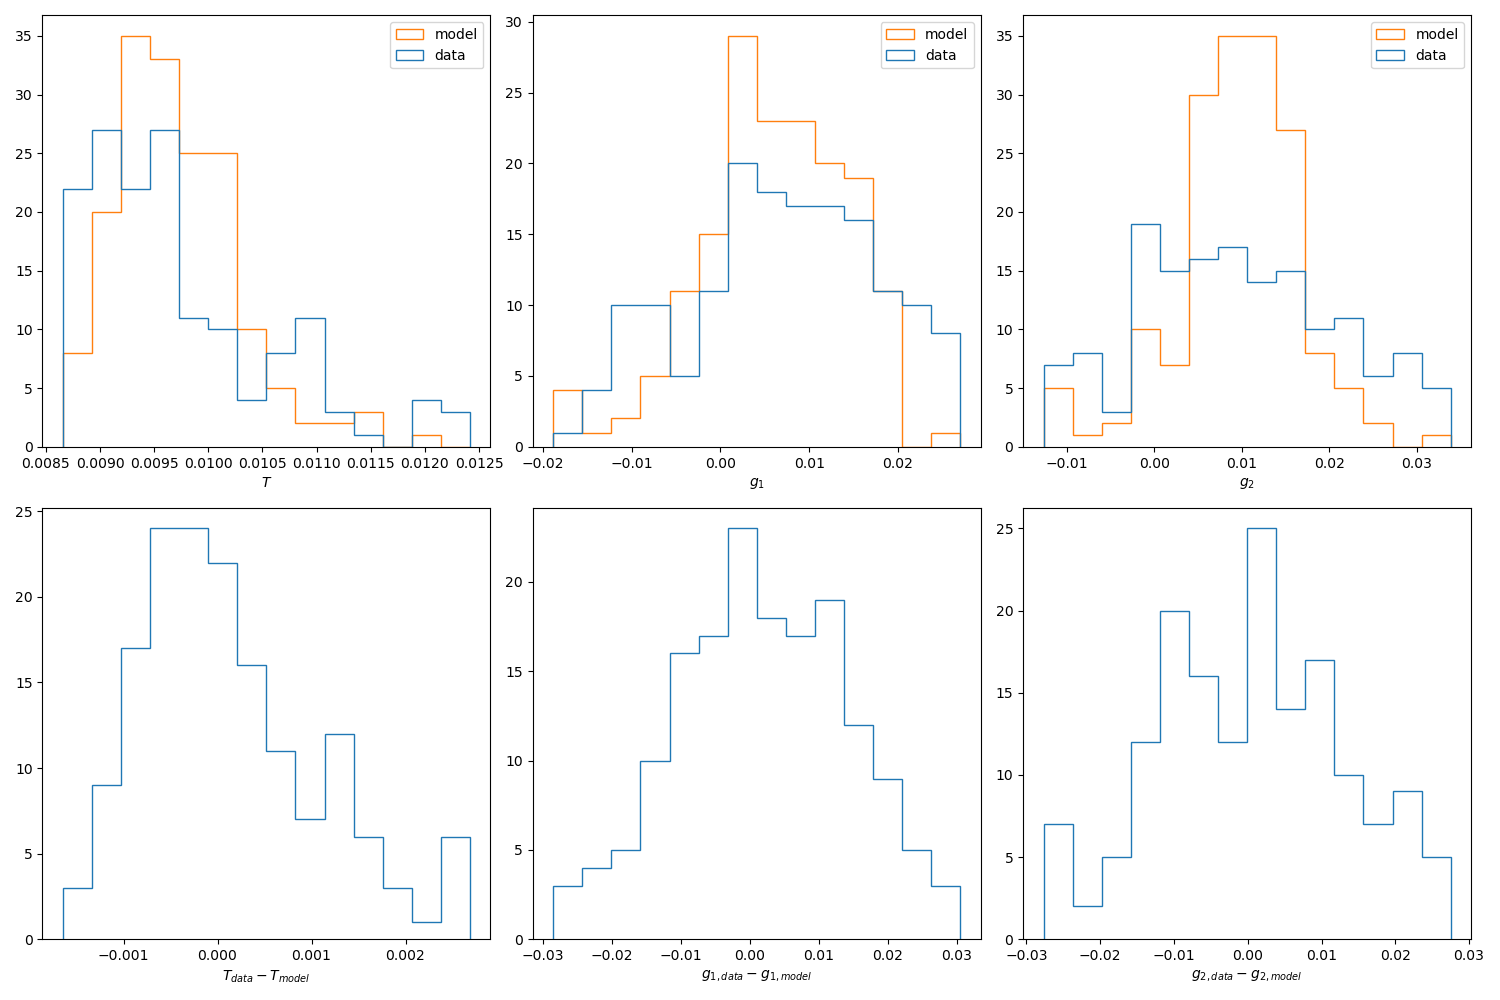
\includegraphics[width=.3\linewidth]{444wOdd/piff_shapes.png}\hfill
  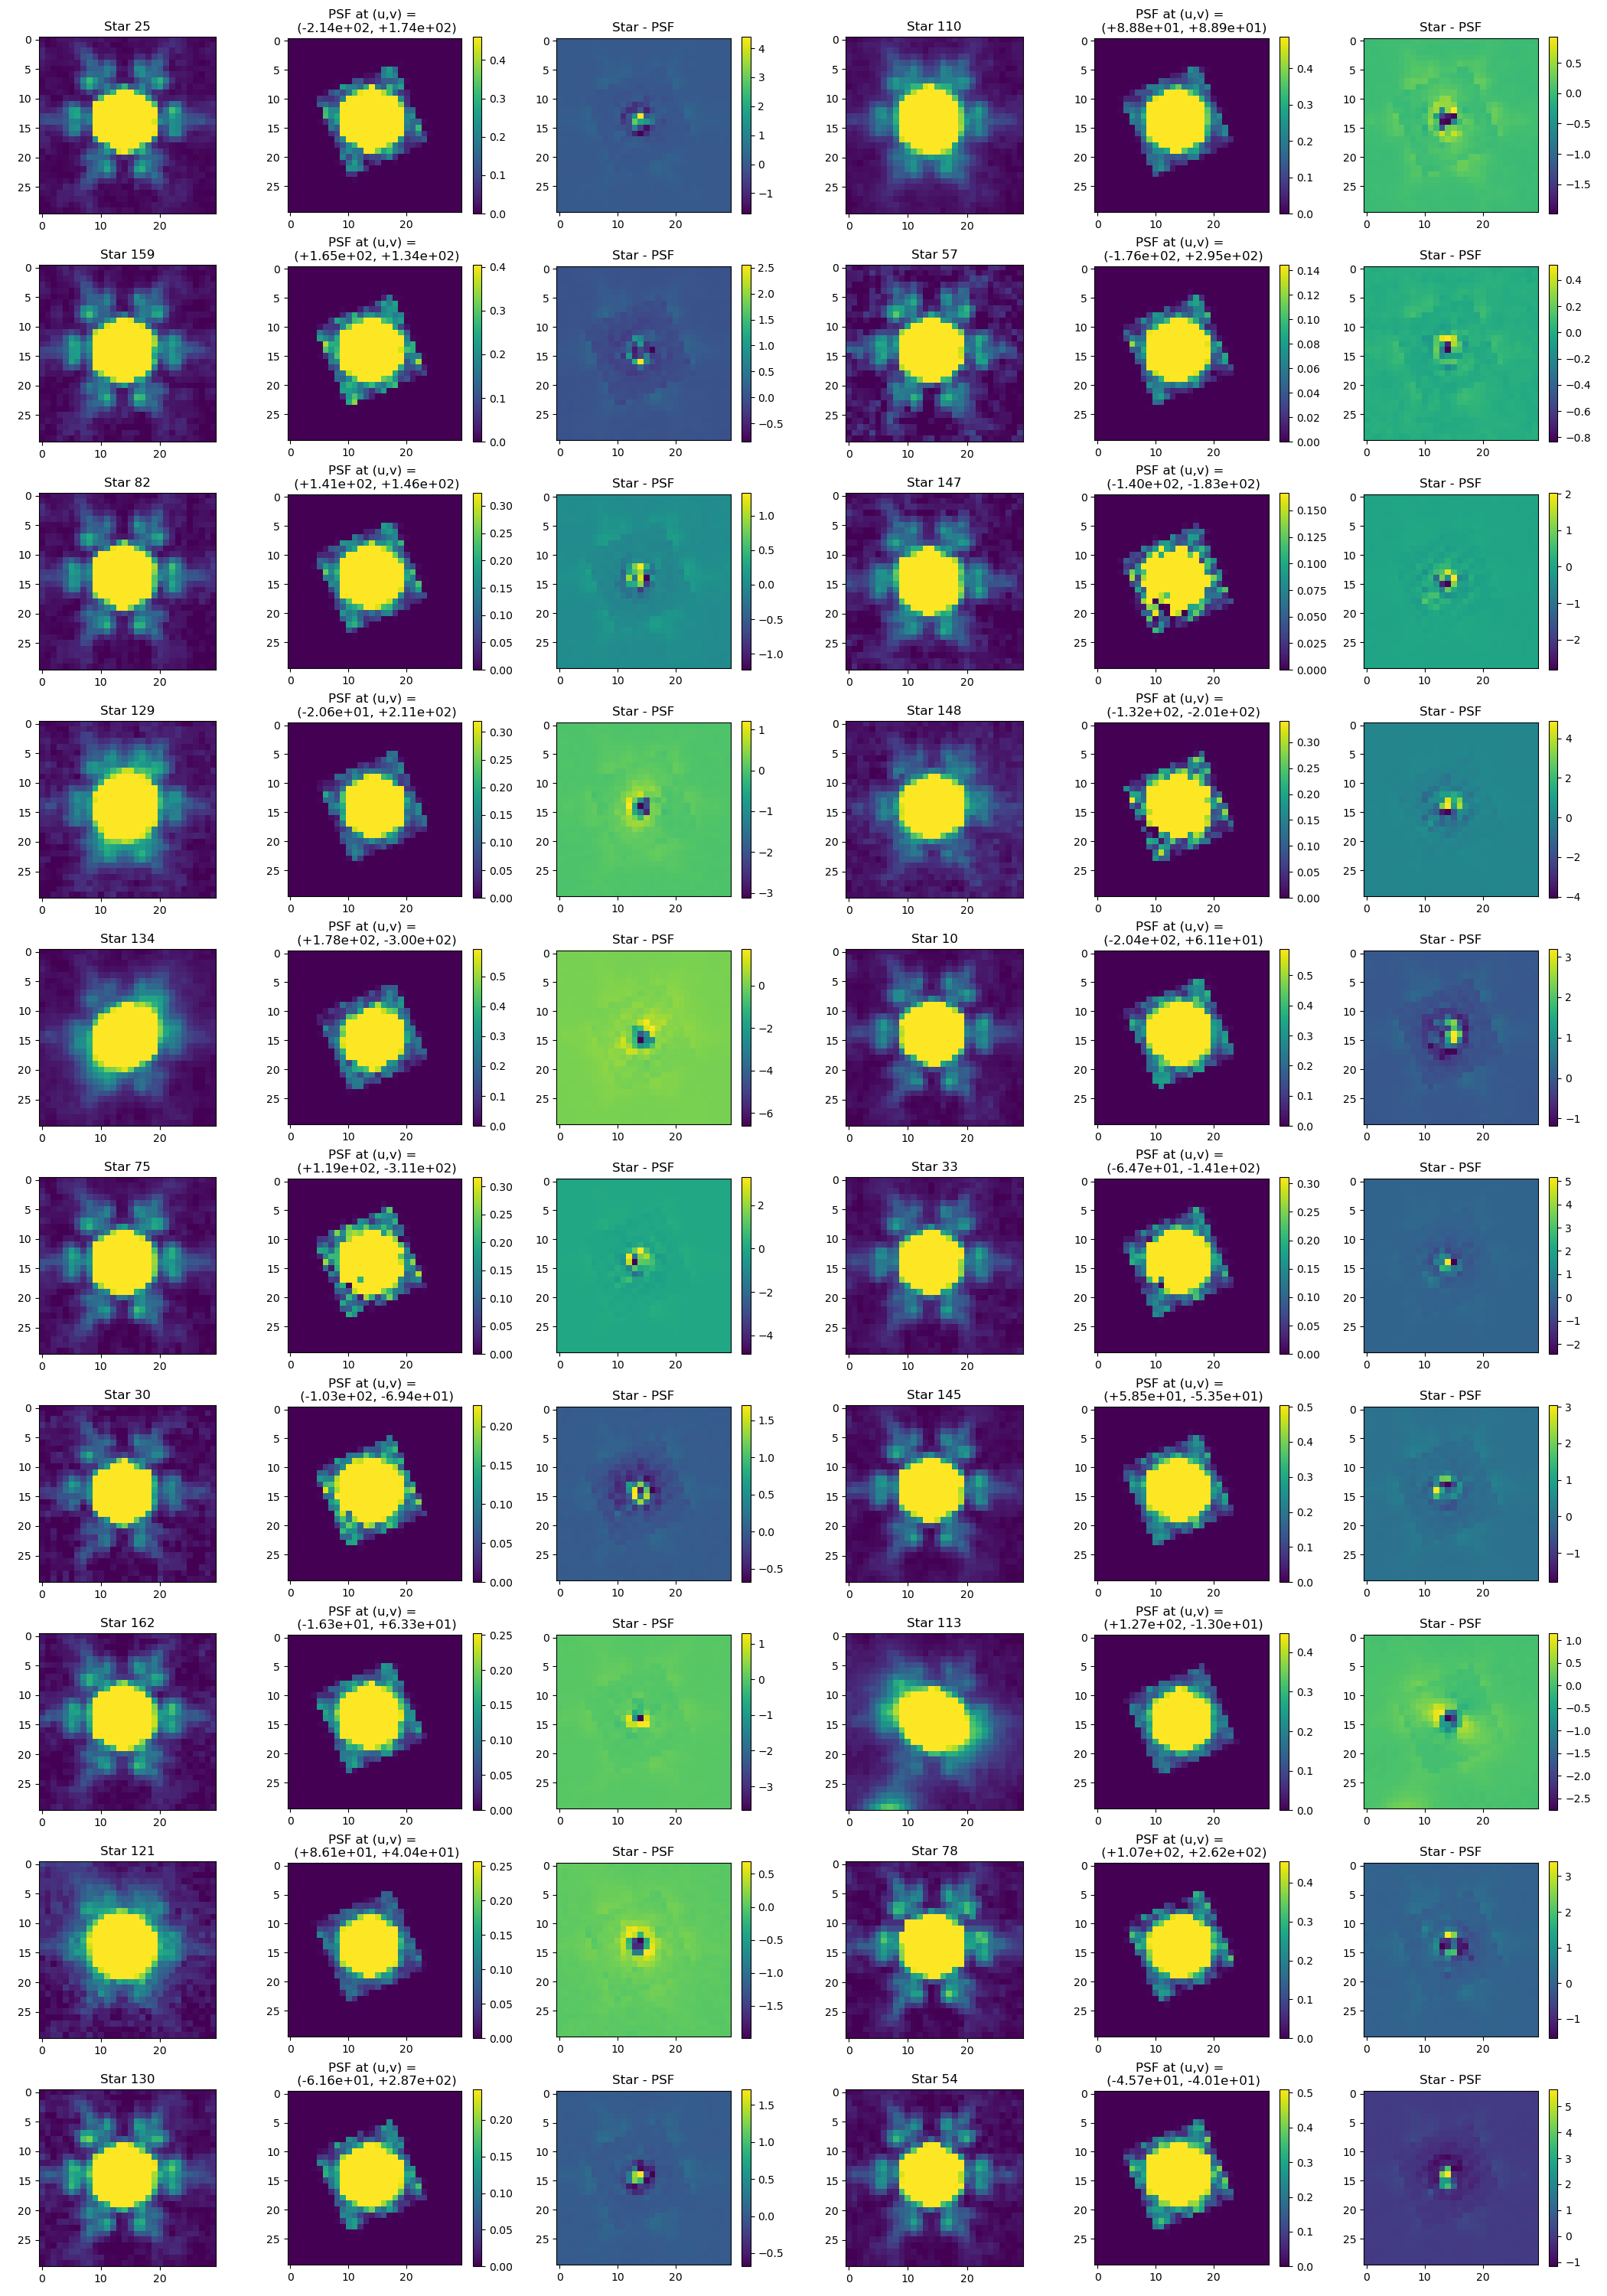
\includegraphics[width=.3\linewidth]{444wOdd/piff_stars.png}
  \end{subfigure}\par\medskip
  \begin{subfigure}{\linewidth}
  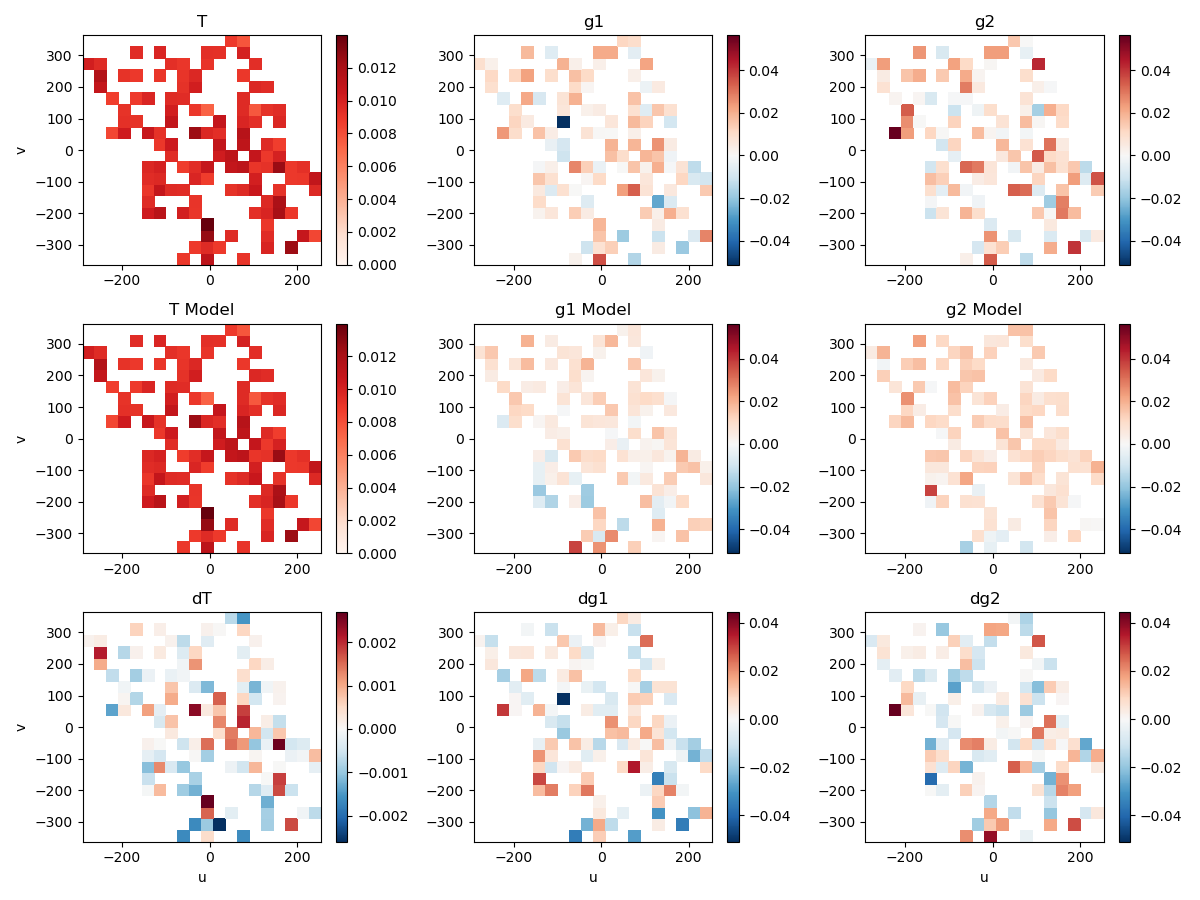
\includegraphics[width=.3\linewidth]{444wOdd/piff_twod.png}\hfill
  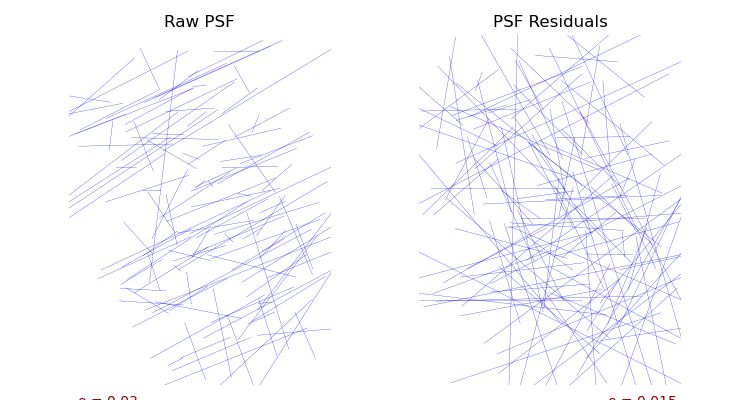
\includegraphics[width=.3\linewidth]{444wOdd/piff_whisker.png}\hfill
  \caption{f444w Odd Model Size}
  \end{subfigure}\par\medskip
\end{figure}\\ \newpage
\\ \clearpage \subsection{Even-Oddness Stamp Size} 
\begin{python}
# How large should the postage stamp cutouts of the stars be?
    stamp_size: 31

model:
    # This model uses a grid of pixels to model the surface brightness distribution.
    type: PixelGrid
    scale: 0.034      # NIRCam ative pixel scale
    size: 26          # Model is 24 x 24 in these pixels
\end{python}\\

\begin{figure}[!h]
  \begin{subfigure}{\linewidth}
  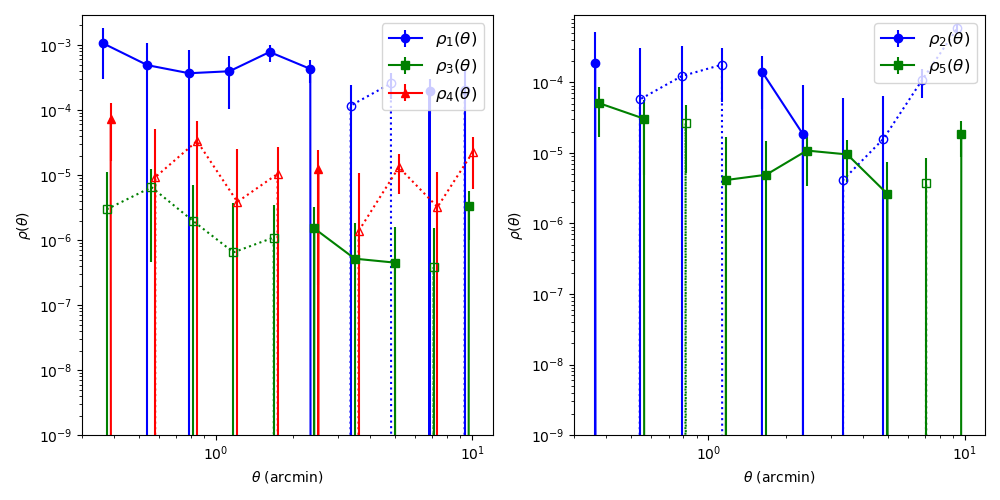
\includegraphics[width=.3\linewidth]{277wStampOdd/piff_rho.png}\hfill
  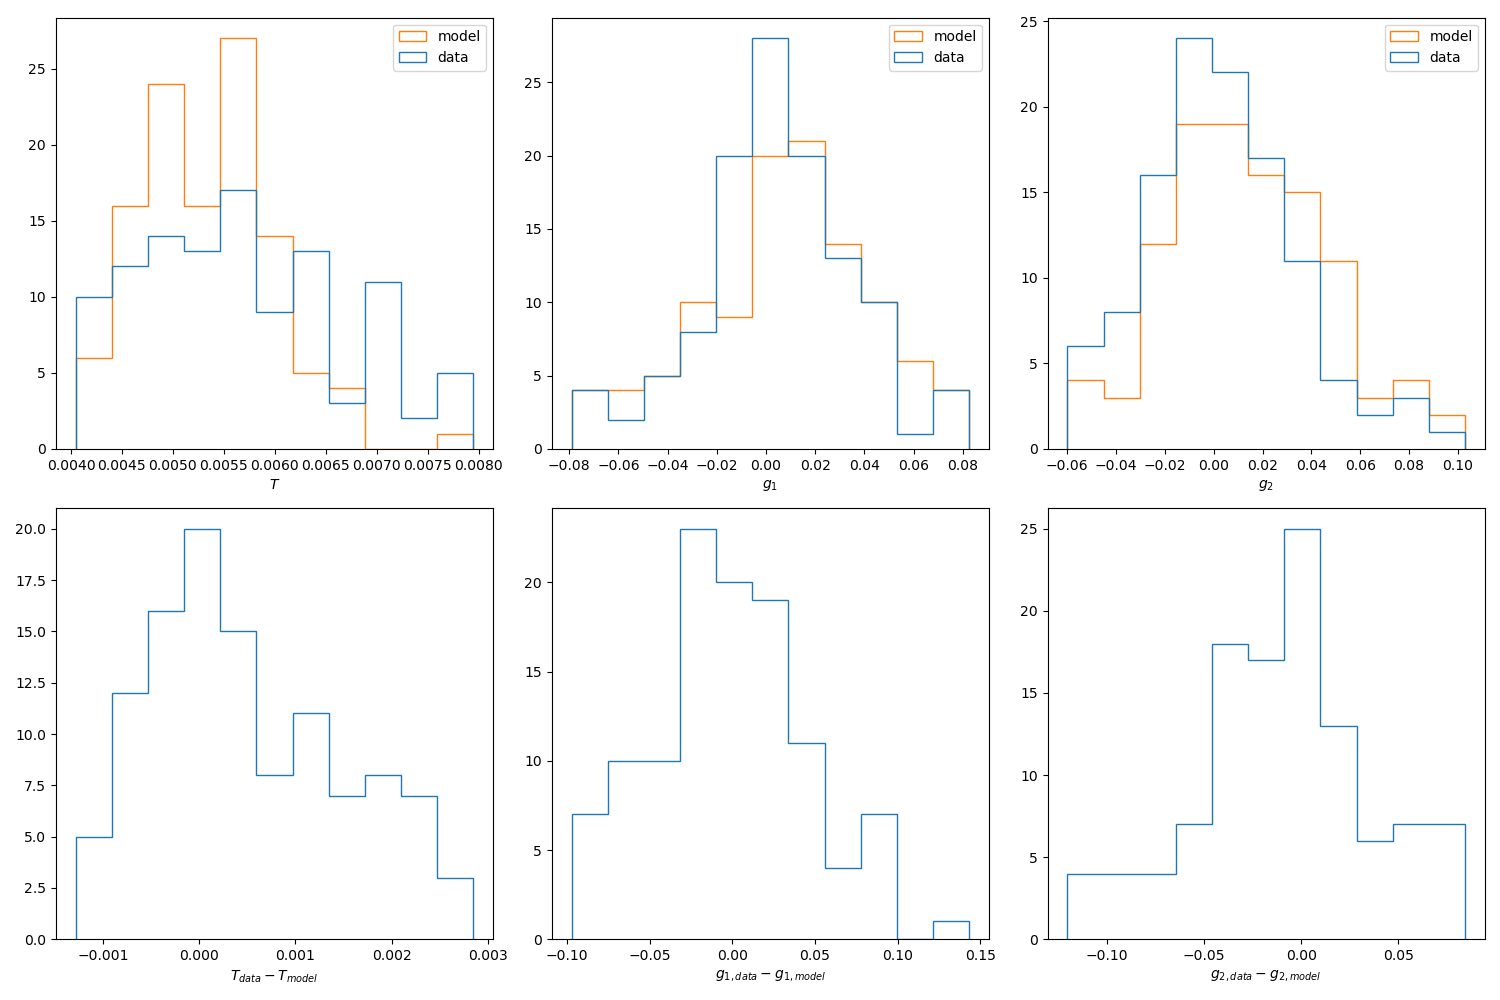
\includegraphics[width=.3\linewidth]{277wStampOdd/piff_shapes.png}\hfill
  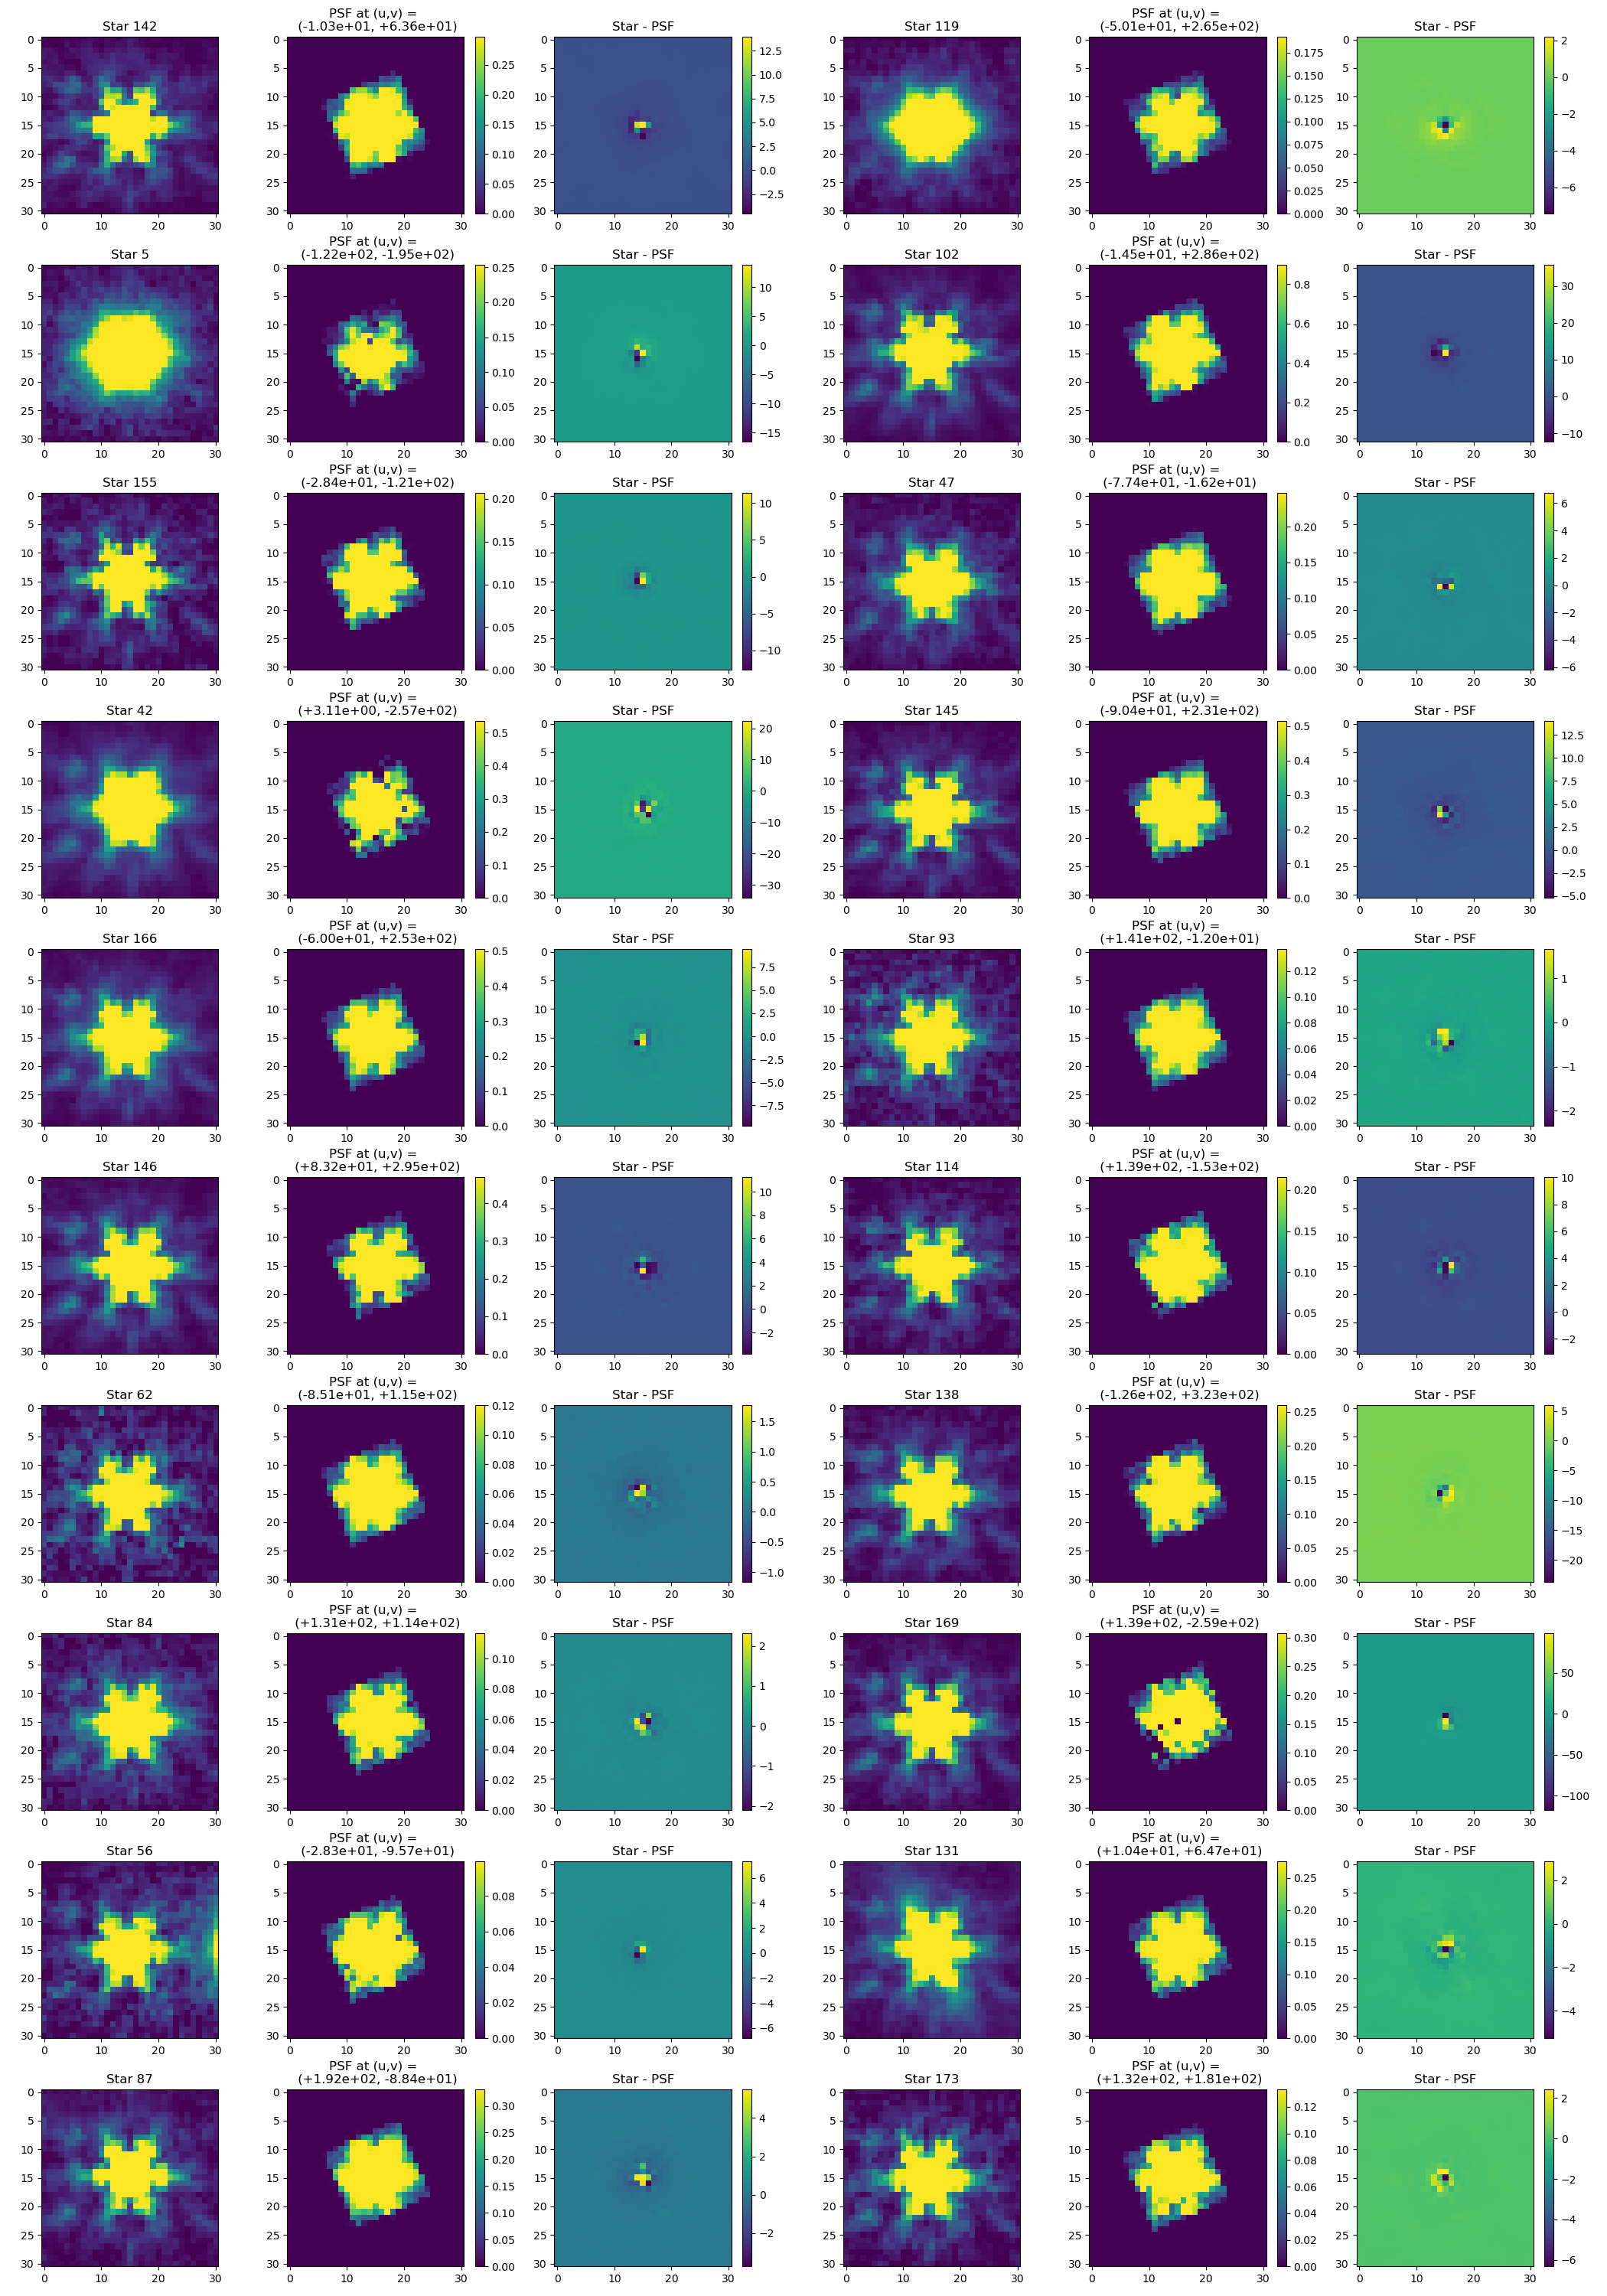
\includegraphics[width=.3\linewidth]{277wStampOdd/piff_stars.png}
  \end{subfigure}\par\medskip
  \begin{subfigure}{\linewidth}
  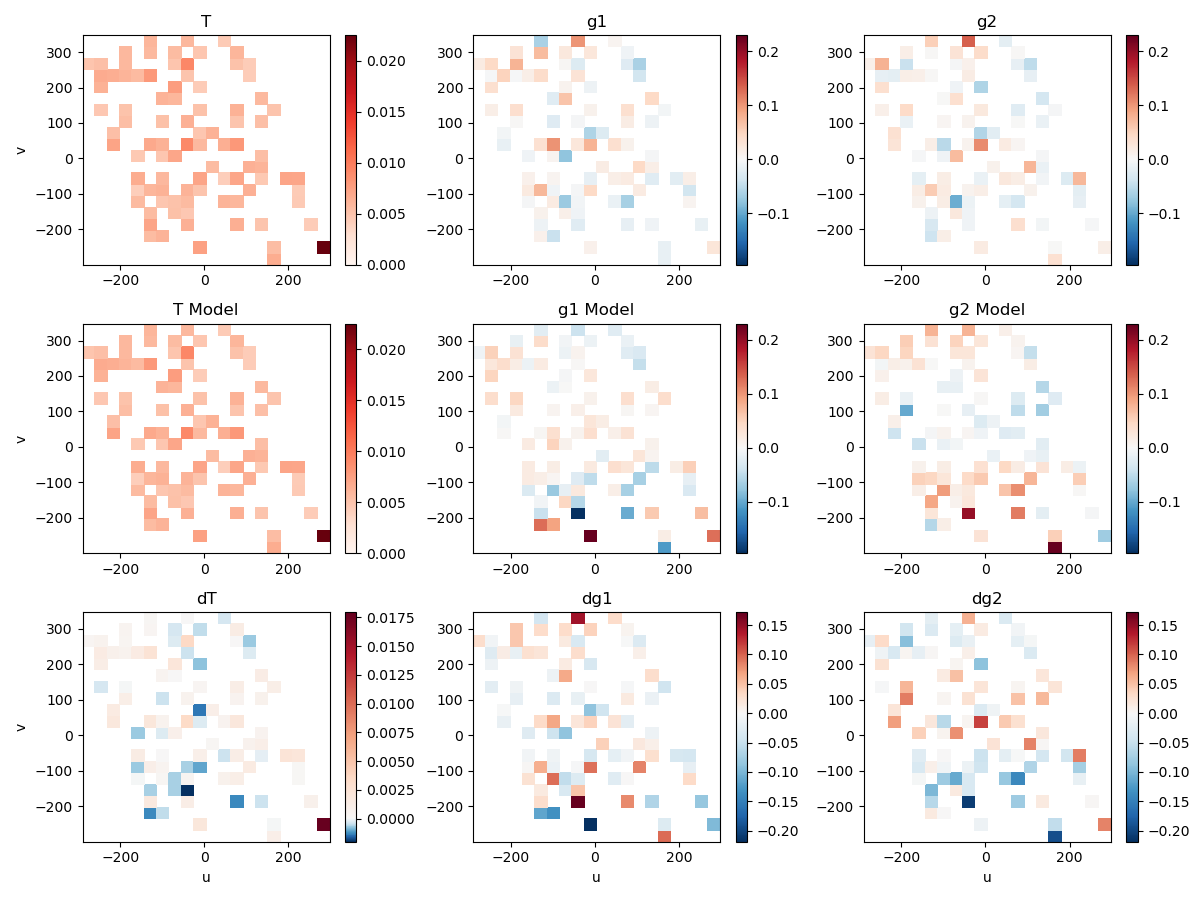
\includegraphics[width=.3\linewidth]{277wStampOdd/piff_twod.png}\hfill
  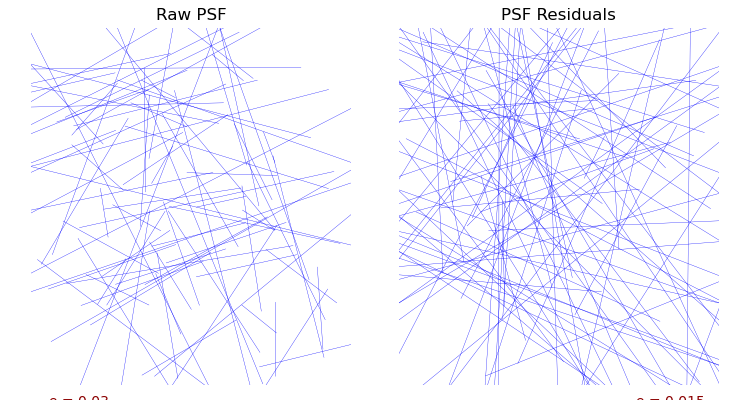
\includegraphics[width=.3\linewidth]{277wStampOdd/piff_whisker.png}\hfill
  \caption{f277w Odd Stamp Size}
  \end{subfigure}\par\medskip
\end{figure}\\
\begin{figure}[!h]
  \begin{subfigure}{\linewidth}
  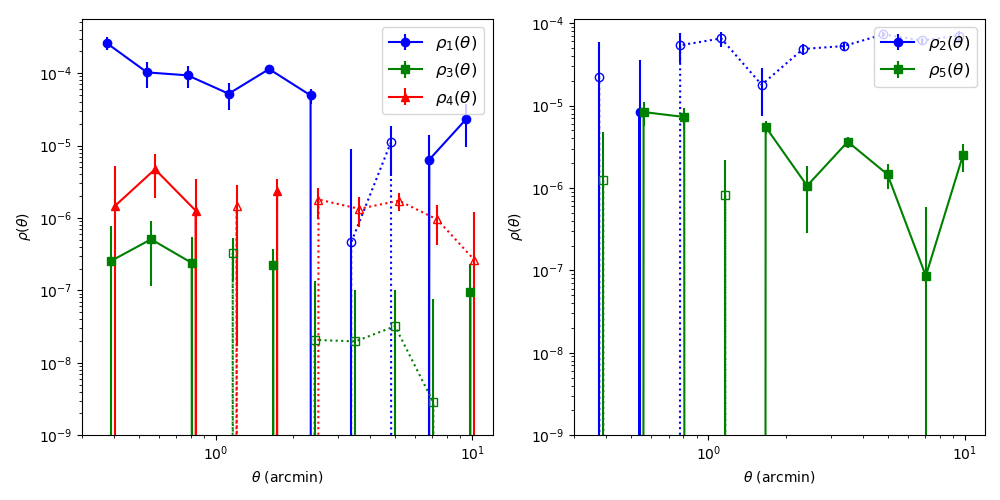
\includegraphics[width=.3\linewidth]{444wStampOdd/piff_rho.png}\hfill
  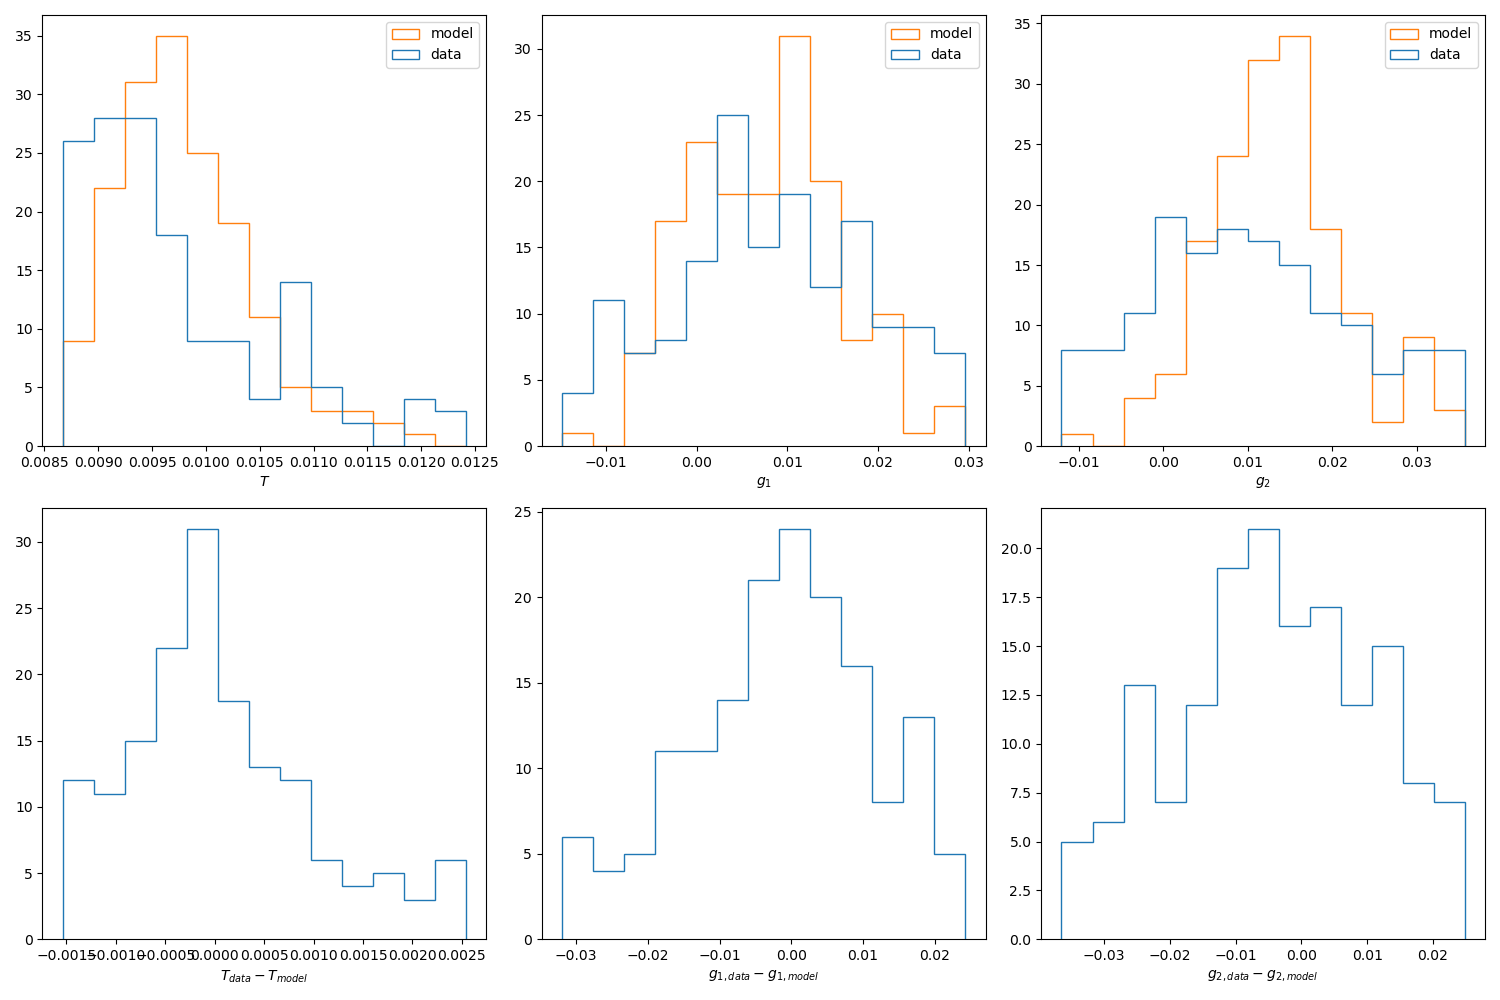
\includegraphics[width=.3\linewidth]{444wStampOdd/piff_shapes.png}\hfill
  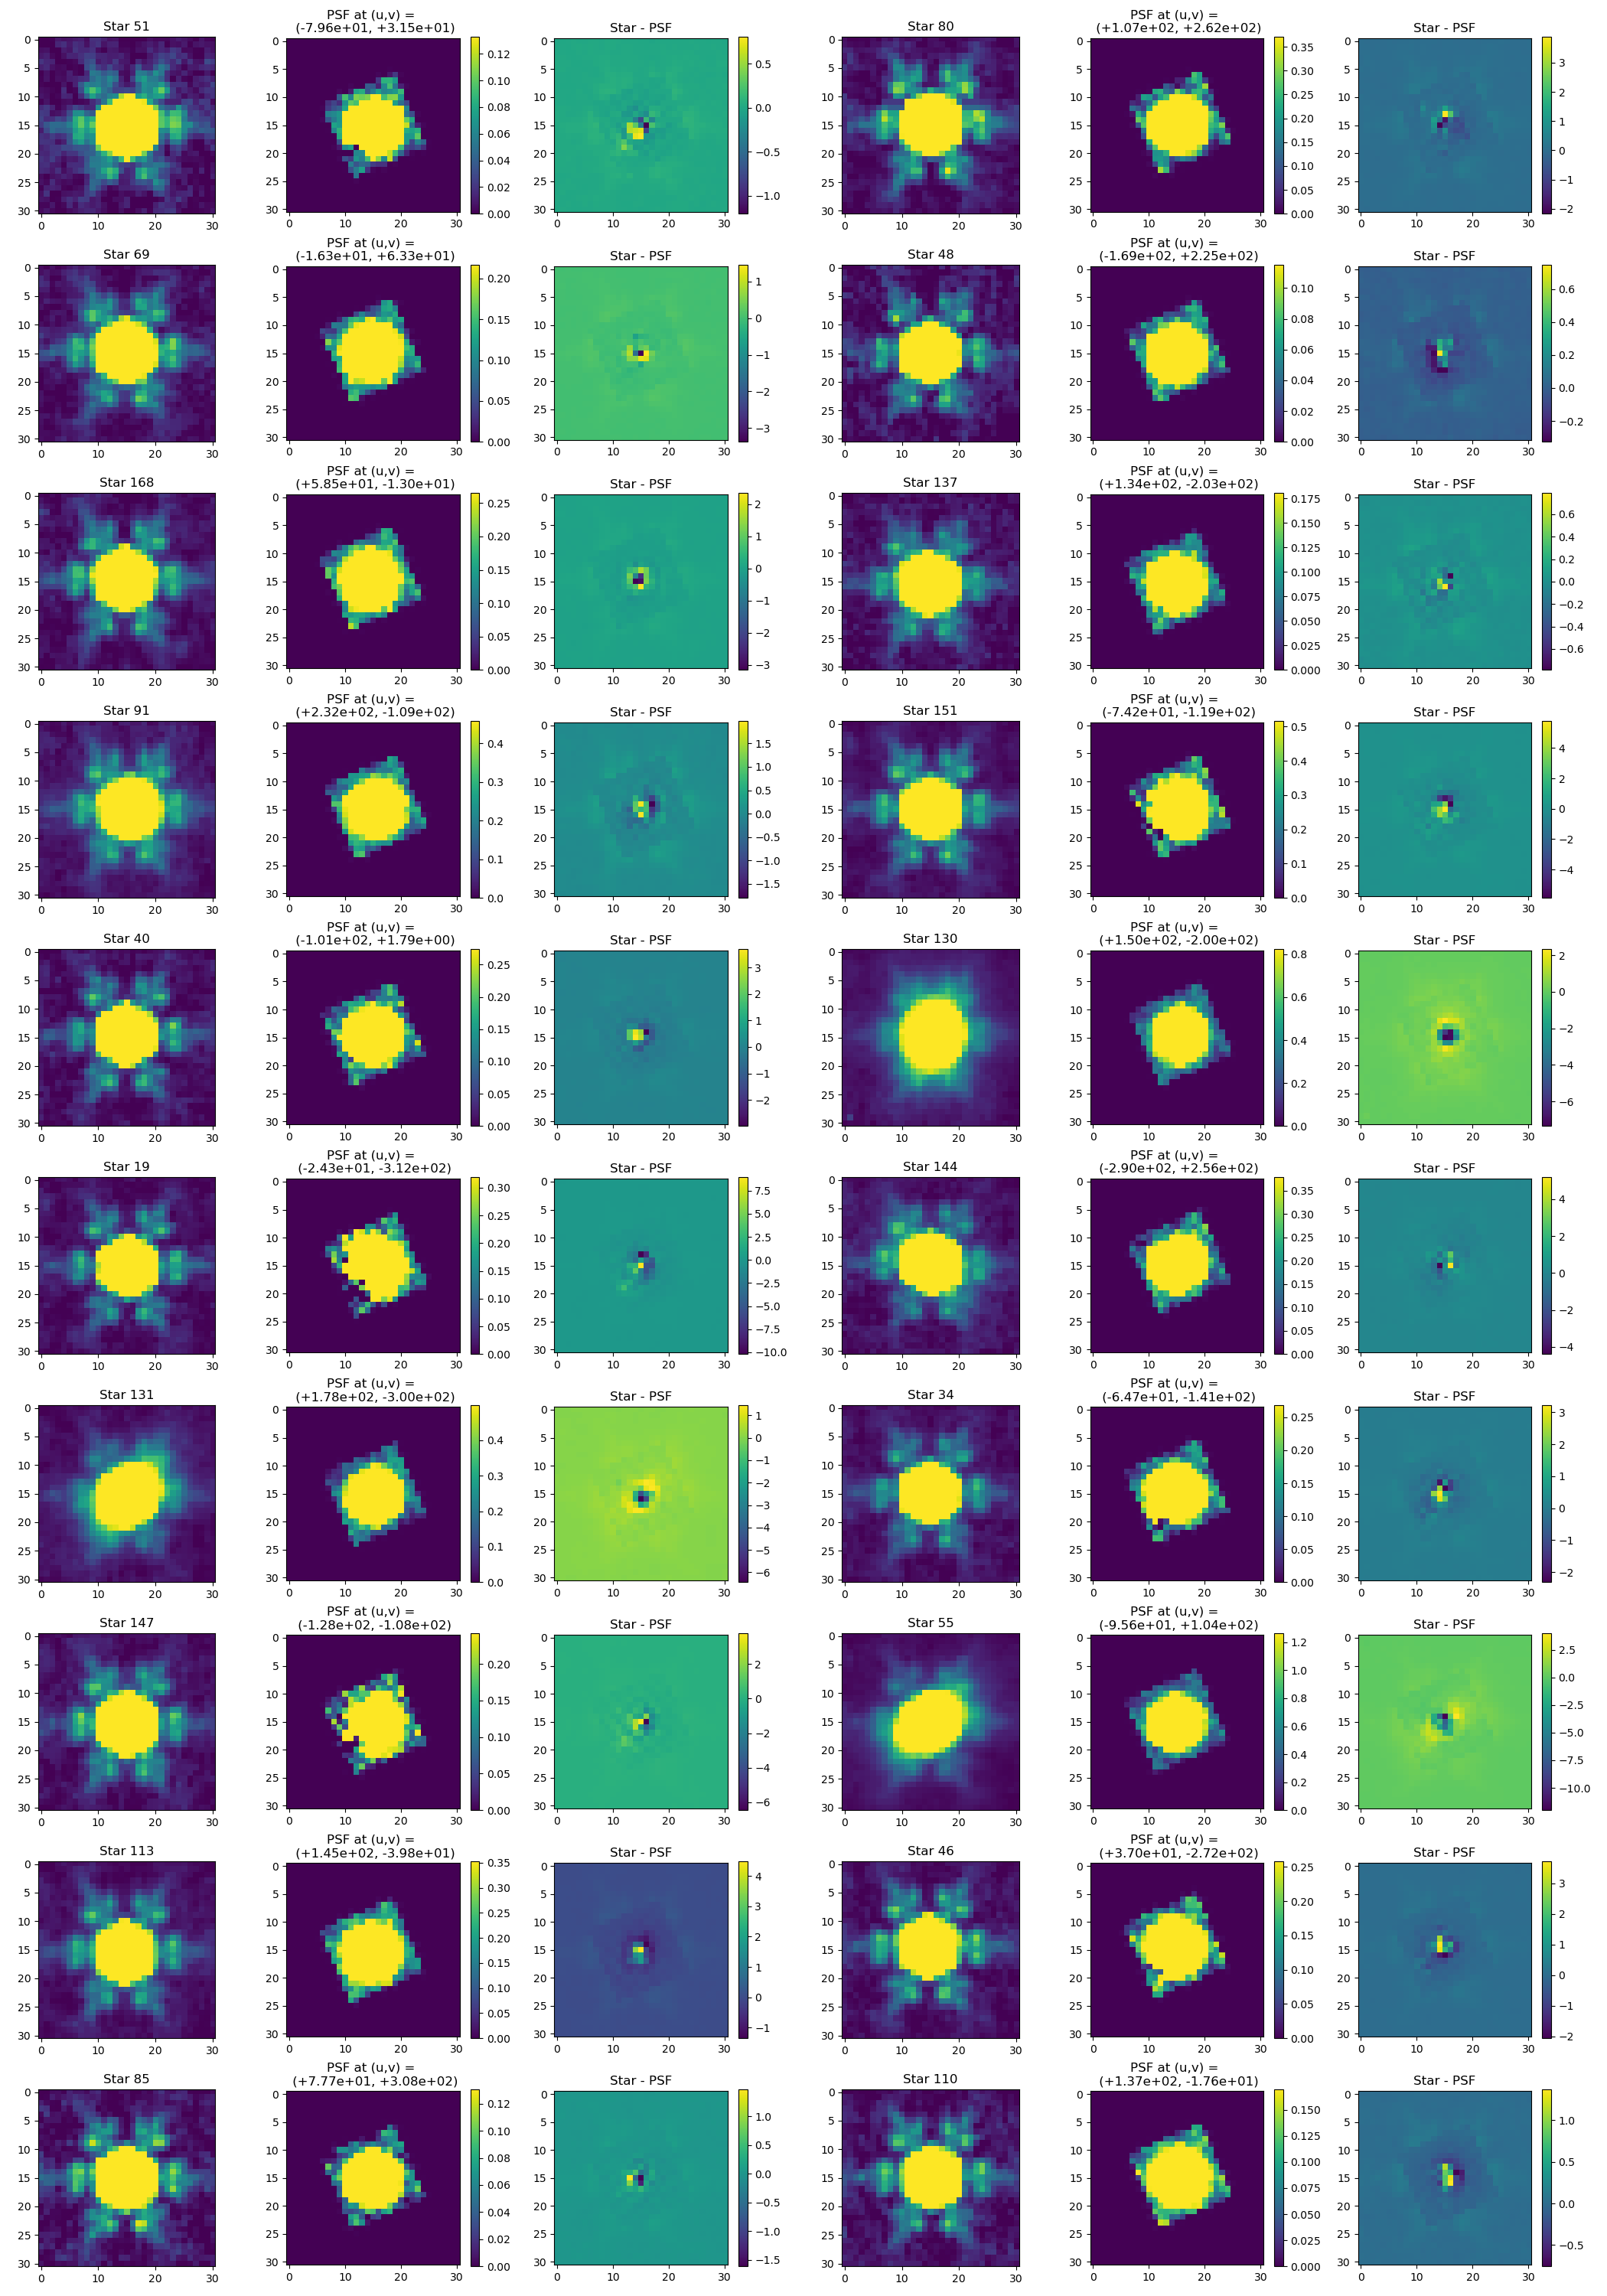
\includegraphics[width=.3\linewidth]{444wStampOdd/piff_stars.png}
  \end{subfigure}\par\medskip
  \begin{subfigure}{\linewidth}
  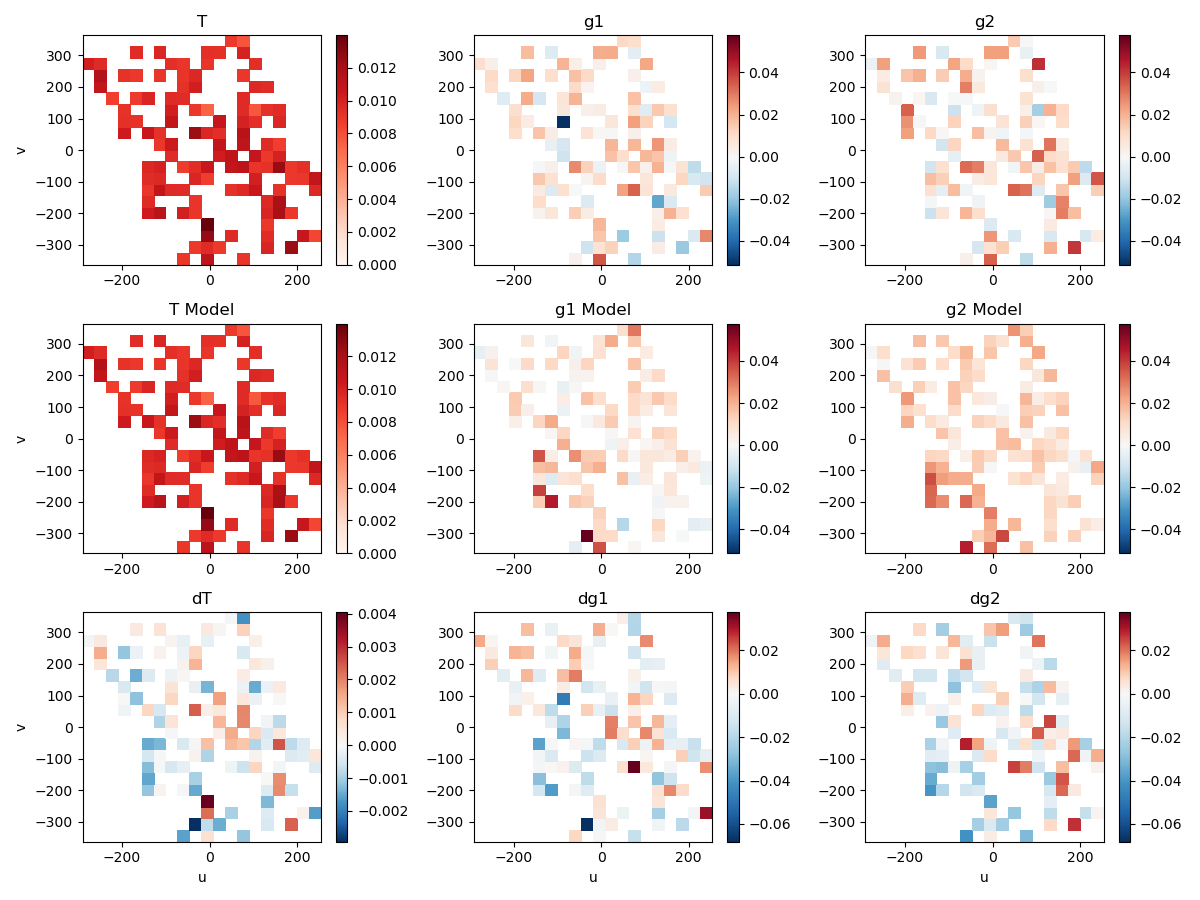
\includegraphics[width=.3\linewidth]{444wStampOdd/piff_twod.png}\hfill
  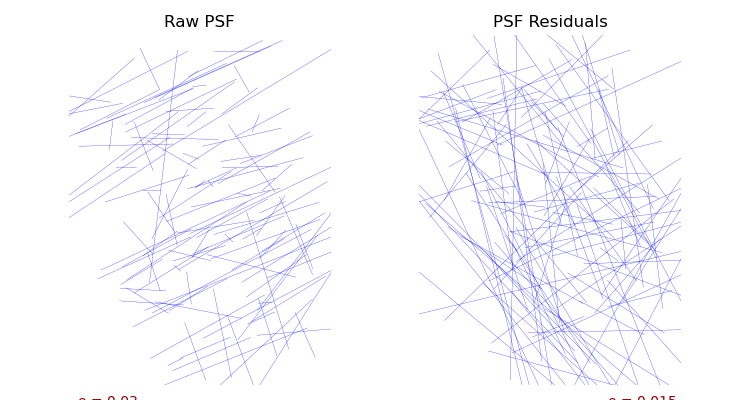
\includegraphics[width=.3\linewidth]{444wStampOdd/piff_whisker.png}\hfill
  \caption{f444w Odd Stamp Size}
  \end{subfigure}\par\medskip
\end{figure}\\
\clearpage \noindent {\fbox{\it Application Process}}\\
\begin{itemize}
    \item All of my rough drafts are done for the Physics Research Co-op Fellowship and Lawrence Research Fellowship 
    \item All files attached below
\end{itemize}
\noindent {\fbox{\it Brown SUMS}}\\ 
\begin{itemize}
    \item There's an upcoming research conference for undergraduates that I alluded to earlier. More information was just released!
    \item \href{https://sites.google.com/brown.edu/sums}{[Here!]}
    \item I am going to explore submitting an abstract and making a powerpoint
    \item I envision something like: Here is all the prerequisite Physics and Math for a broader audience. Some fun images of the telescope I am modeling, per the Nircam documentation you sent me. Here is what I've explored, I now have lots of images that I can use to show off my findings. Here are some known issues. Now, future direction!
\end{itemize}\\
\noindent {\fbox{\it A Curious Paper}}\\ 
\begin{itemize}
    \item I came across an interesting paper that really piqued my interest because it combines lots of your background with things closer to my background and so I wanted to share it
    \item \href{https://arxiv.org/abs/2103.09247}{[Here!]}
\end{itemize}\\
\noindent {\fbox{\it Slack and Meetings}}\\ 
\begin{itemize}
    \item You mentioned last time it would be good for me to go to the weekly meetings for our collaboration. I would love to start attending but I think that requires me to get integrated with Slack.
\end{itemize}
\noindent {\fbox{\it My Workshop}}\\ 
\begin{itemize}
    \item My club, the Mathematics Engagement and Mentorship Association, is in the planning phases of our first ever introductory workshop on how to read a research paper
    \item I was wondering if you had any messages about reading papers that may be of use to our mentees (and me as well, I still have a ways to go)
\end{itemize}
\noindent {\fbox{\it Keyboard}}\\ 
\begin{itemize}
    \item Our last meeting you offered to buy some peripherals for me to use with some of the money you got for your labspace. A keyboard with the default settings found here would be great \href{https://system76.com/accessories/launch_lite_sa_1/configure}{[Keyboard Link]}
\end{itemize}
\noindent {\fbox{\it Summer 1 Plans}}\\ 
\begin{itemize}
    \item Either classes or the RTG. Either way, I'll be around to do work.
\end{itemize}
\noindent {\fbox{\it Class Observations}}\\ 
\begin{itemize}
    \item Learned in class about some issues with optimization on ellipses, maybe pertinent
\end{itemize}
\noindent {\fbox{\it Still to Do}}\\ 
\begin{itemize}
    \item I'd like to parse through the PIFF documentation to reverse engineer it, I've been thinking a lot about the problem and I think for me to start attempting my own I need a stronger mathematical framework for what it is doing
    \item This seems to give me some idea \href{http://rmjarvis.github.io/Piff/_build/html/model.html}{[Here]}
    \item PSF beyond an operational definition
\end{itemize}
\newpage
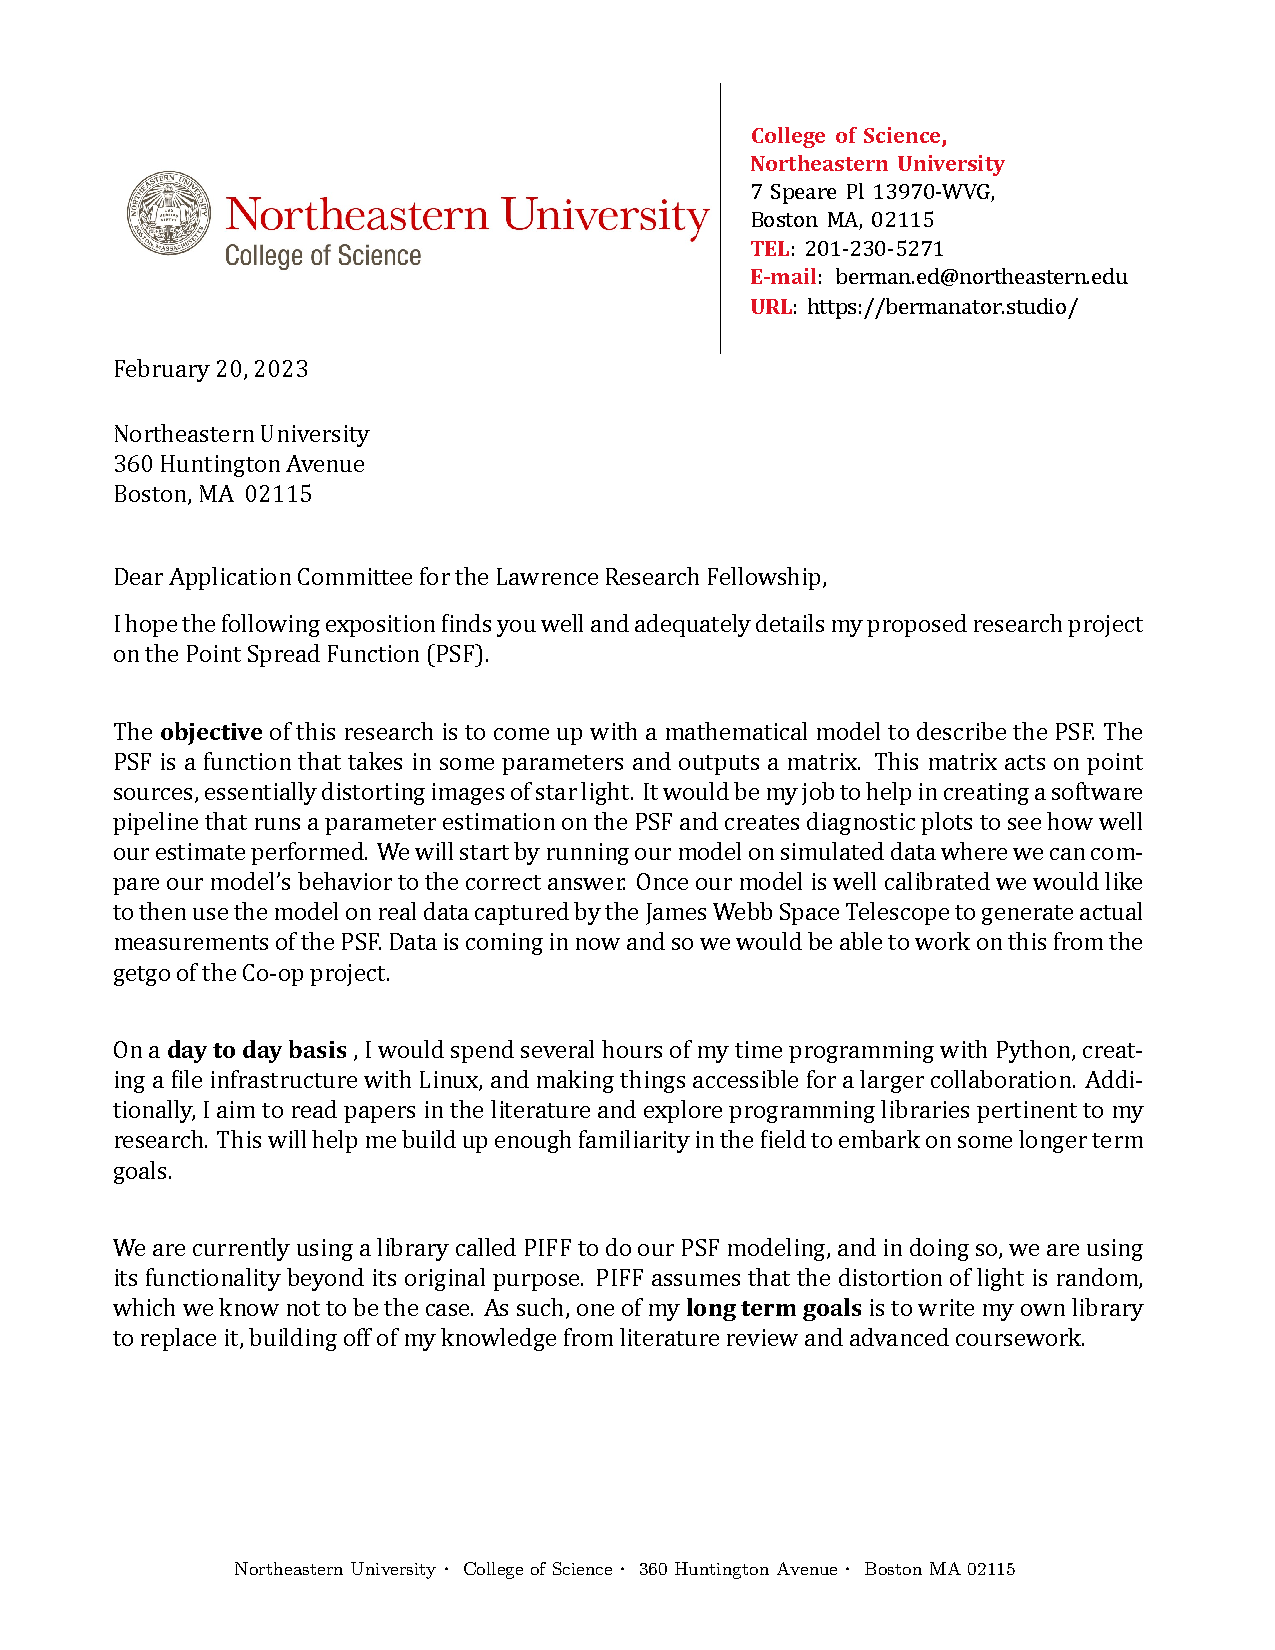
\includepdf[pages=-]{Lawrence_Research_Fellowships.pdf}

\includepdf[pages=-]{Cover_Letter_Physics_Research_Co_op_Fellowships.pdf}
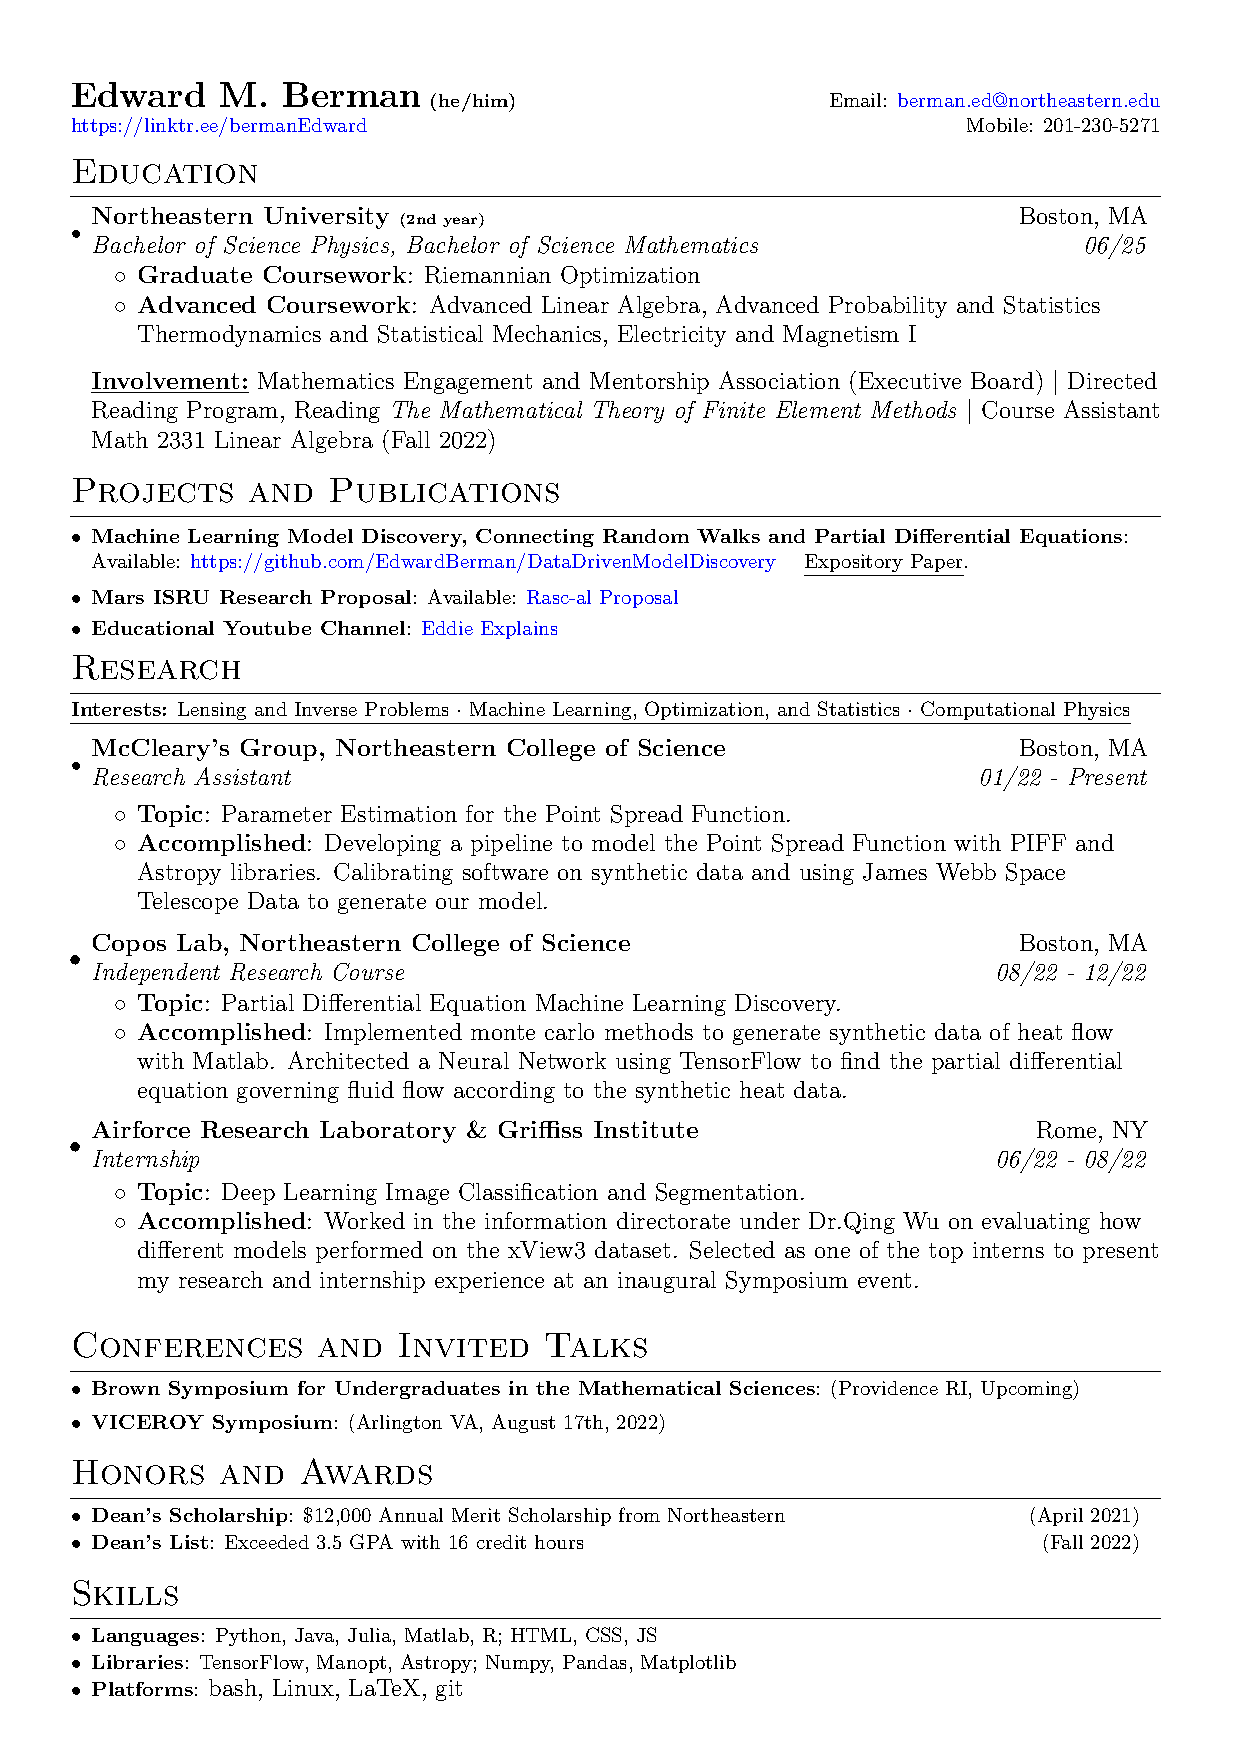
\includepdf[pages=-]{Resume_CV_Northeastern_COOP_Grant__Resume.pdf}
\newpage

















\end{document}
%%------------ Arman Shokrollahi--------------%%
